%!TEX root = thesis.tex
\chapter{Results}\label{chap:results}
\thispagestyle{plain}

  This chapter details all performed experiments and presents their results. All experiments run the implemented \vas{} model in a variety of setting and compare it to the flowline model. The focus is on the intrinsic model behavior and its comparison to the flowline model, and with the exception of the final projection experiment less on absolute ice volume estimations. The experiments start with a test run performed on six different single glacier (Section~\ref{sec:single_glacier_test_case_results}), including time series analysis investigating autocorrelation functions and power spectral density (Section~\ref{sec:autocorrelation_and_power_spectral_density_results}). The same equilibrium runs are repeated on a regional scale (Section~\ref{sec:regional_runs_with_all_alpine_glaciers_results}), before looking into the model's sensitivities to its scaling parameters (Section~\ref{sec:sensitivity_experiments_results}).
  The final experiment runs projections over the 21st century for Central Europe and High Mountain Asia (Section~\ref{sec:projections_for_the_21st_century}).

  \section{Single glacier test case} % (fold)
  \label{sec:single_glacier_test_case_results}

    The first qualitative look at the performance of the \vas{} model uses the Hintereisferner (RGI60-11.00897) as a test case. This test case is intended to get a feel for the model and set the stage for the following experiments, by comparing two evolution models and the two mass balance models. 
    It has to be noted, that applying \vas{} to a single glacier gives only an order of magnitude estimate. The scaling constant $c$ is a globally averaged value, and the relative error in scaling constant is directly proportional to the error in estimated ice volume \citep{Bahr2015}. However, a qualitative comparison between the \vas{} model and the flowline model is more practicable and meaningful for a single glacier. The model's sensitivity to its scaling parameters is investigated in Section~\ref{sec:sensitivity_experiments_results}. Additionally, the same experiment is repeated for five more glaciers with similar results shown in Appendix~\ref{appendix_A}.

    \begin{tldrbox}[Single glacier test case]{tldr:hintereisferner_test_case_results}
      \item Both evolution models produce the same qualitative results, advancing under colder climates and shrinking under warmer climates. The temporal correlation between both models under a random climate is satisfying.
      \item The \vas{} model estimates much smaller changes in glacier geometry compared to the flowline model (up to four times). For example, the relative volume changes for the run with positive mass balance bias amount to $\SI{+17}{\percent}$ for the \vas{} model and $\SI{+71}{\percent}$ for the flowline model. 
      \item The \vas{} does not account for the mass-balance-elevation feedback and therefore produces highly symmetrical results between the positive and negative step change in air temperature. This symmetry can also be seen in the e-folding response times.
      \item The e-folding response times are much shorter for the \vas{} model. For example, the volume response times for the run with positive mass balance bias amount to $\SI{39}{\year}$ for the \vas{} model and $\SI{139}{\year}$ for the flowline model. 
      \item The \vas{} model does not show an asymptotic adjustment but behaves more like a damped harmonic oscillator, whereby the model-internal time scale acts as damping factor.
    \end{tldrbox}
    
    \subsection{Experimental setup} % (fold)
    \label{sub:experimental_setup_test_case}

        % Mass balance calibration and mass balance models using the same tstar
        For this first experiment, both evolution models run with the \lstinline`ConstantMassBalance` model and the \lstinline`RandomMassBalance` model, for 1000 years each. Both mass balance models emulate an equilibrium climate to keep the glacier in its initial equilibrium state. Therefore, the mass balance models must be initialized with the climatic period centered around the equilibrium year, i.e., \lstinline`y0` = \tstar{}. As explained above, the mass balance calibration depends among other parameters on \tstar{} (Section~\ref{sub:temperature_index_model}, see \hyperref[ssub:mb_calib]{Calibration of the mass balance parameters}). Hence, to run both evolution models with the identical climatic forcing, \tstar{} must be equal for both. This is done by using the same \tstar{} reference table (\lstinline`oggm_ref_tstars_rgi6_histalp.csv`, corresponding to the flowline model) to compute the temperature sensitivity \mustar{} for both models . Additionally, the mass balance residual must be omitted during the model run ($\beta^*$ = 0, as by the definition of \mustar{}, see Section~\ref{sub:temperature_index_model}). Each mass balance model runs three different climate scenarios defined by respective the temperature bias of \SI{0}{\celsius}, \SI{-0.5}{\celsius} and \SI{+0.5}{\celsius}. This results in a equilibrium run, a run with positive mass balance perturbation and a run with negative mass balance perturbation, respectively.

    % subsection experimental_setup (end)

    \subsection{Results} % (fold)
    \label{sub:results_test_case}

        % Figure showing Hintereisferner time series plots - on page
        \begin{figure}[p]
          \centering

          % VAS volume
          \begin{subfigure}[b]{0.476\textwidth}
            \caption{\Vas{} model, relative ice volume}
            \label{fig:hintereisferner:volume_vas}
            \centering
            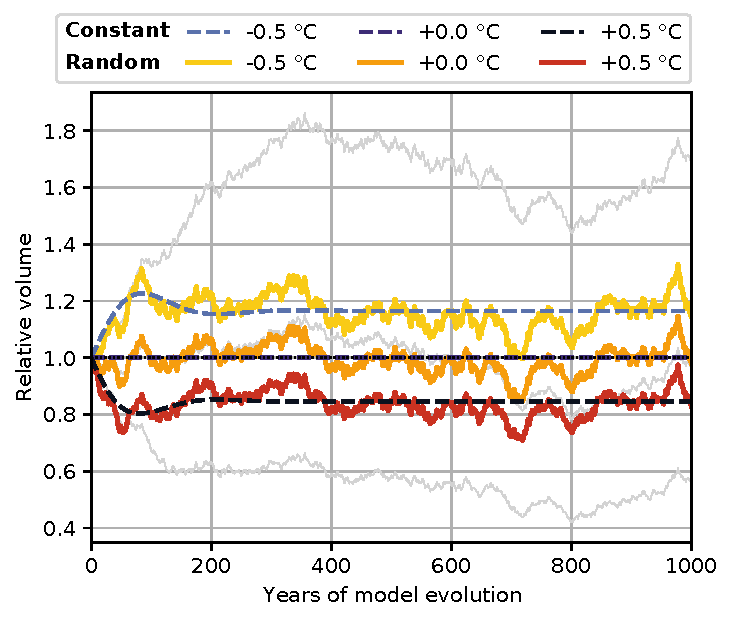
\includegraphics[width=\textwidth]{../plots/final_plots/time_series/single_glaciers/volume_norm_vas_Hintereisferner.pdf}
          \end{subfigure}
          \hfill
          % Flowline volume
          \begin{subfigure}[b]{0.476\textwidth}
            \caption{Flowline model, relative ice volume}
            \label{fig:hintereisferner:volume_fl}
            \centering
            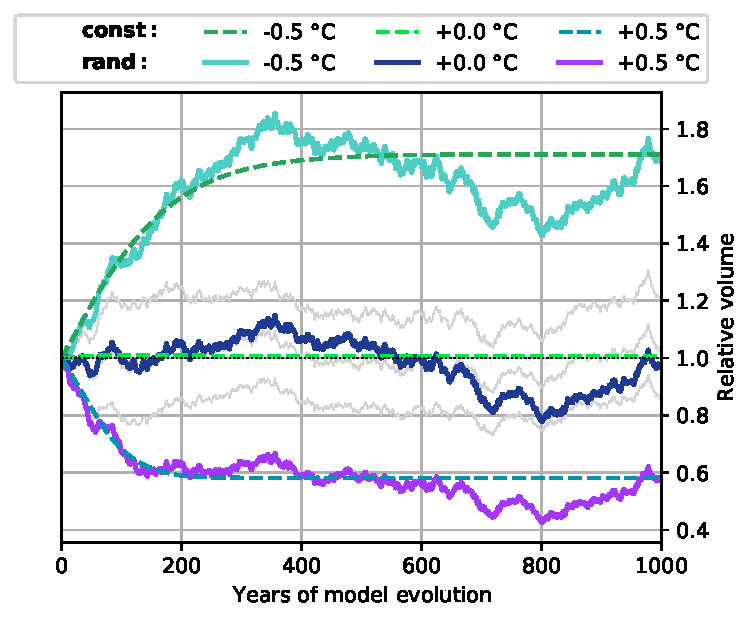
\includegraphics[width=\textwidth]{../plots/final_plots/time_series/single_glaciers/volume_norm_fl_Hintereisferner.pdf}
          \end{subfigure}

          % VAS area
          \begin{subfigure}[b]{0.476\textwidth}
            \caption{\Vas{} model, relative surface area}
            \label{fig:hintereisferner:area_vas}
            \centering
            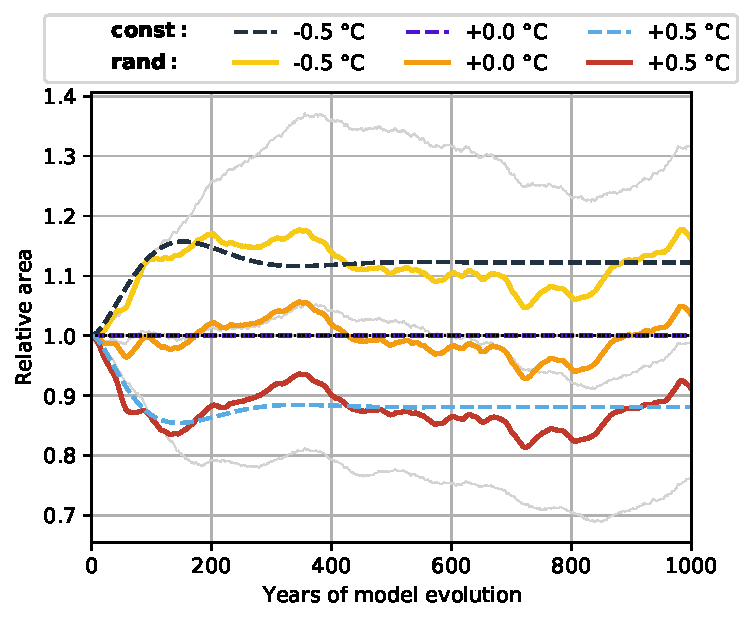
\includegraphics[width=\textwidth]{../plots/final_plots/time_series/single_glaciers/area_norm_vas_Hintereisferner.pdf}
          \end{subfigure}
          \hfill
          % Flowline area
          \begin{subfigure}[b]{0.476\textwidth}
            \caption{Flowline model, relative surface area}
            \label{fig:hintereisferner:area_fl}
            \centering
            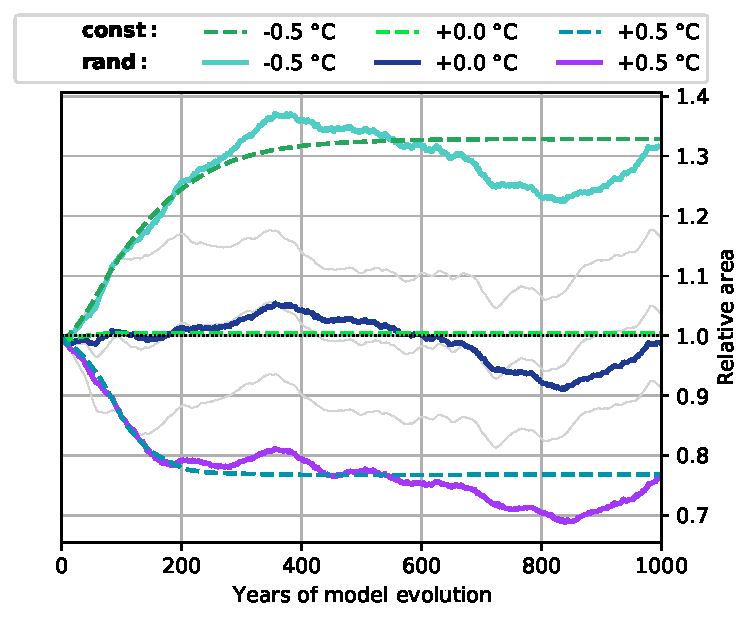
\includegraphics[width=\textwidth]{../plots/final_plots/time_series/single_glaciers/area_norm_fl_Hintereisferner.pdf}
          \end{subfigure}

          % VAS length
          \begin{subfigure}[b]{0.476\textwidth}
            \caption{\Vas{} model, relative glacier length}
            \label{fig:hintereisferner:length_vas}
            \centering
            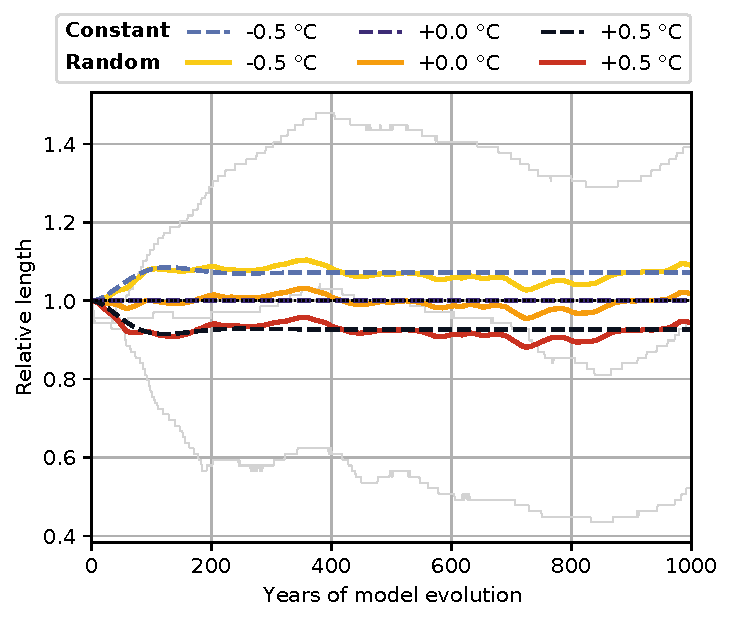
\includegraphics[width=\textwidth]{../plots/final_plots/time_series/single_glaciers/length_norm_vas_Hintereisferner.pdf}
          \end{subfigure}
          \hfill
          % Flowline length
          \begin{subfigure}[b]{0.476\textwidth}
            \caption{Flowline model, relative glacier length}
            \label{fig:hintereisferner:length_fl}
            \centering
            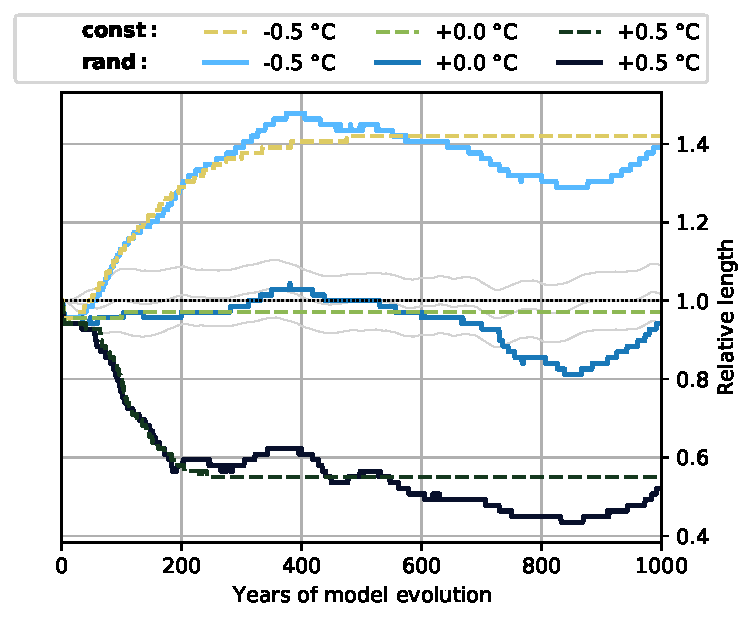
\includegraphics[width=\textwidth]{../plots/final_plots/time_series/single_glaciers/length_norm_fl_Hintereisferner.pdf}
          \end{subfigure}
          
          \caption{Temporal evolution of ice volume in (\subref{fig:hintereisferner:volume_vas}) and (\subref{fig:hintereisferner:volume_fl}), surface area in (\subref{fig:hintereisferner:area_vas}) and (\subref{fig:hintereisferner:area_fl}) and glacier length in (\subref{fig:hintereisferner:length_vas}) and (\subref{fig:hintereisferner:length_fl}) for Hintereisferner (RGI60-11.00897). The shown values area normalized with their respective initial values. The left panels show the result of the \vas{} model, the right panels show the results of the flowline model. Solid lines represent the random climate scenarios, while dashed lines represent the constant climate scenarios. All climate scenarios are based on an equilibrium climate. The applied temperature biases of \SI{-.5}{\celsius}, \SI{0}{\celsius} and \SI{+.5}{\celsius} are color coded, see legend for details. The dotted line indicates the initial volume. The light gray lines represent the volume evolutions of the other model, to facilitate comparisons.}
          \label{fig:hintereisferner}
        \end{figure}

        % overall impression
        Figure~\ref{fig:hintereisferner} shows the temporal evolution of relative ice volume, surface area and glacier length for Hintereisferner, comparing both mass balance models (solid vs. dashed lines) and both evolution models (left vs. right panels). The \vas{} model behaves as expected and produces the same qualitative results as the flowline model. The model glacier stays in an approximate equilibrium using the climate around \tstar, and decreases and increases in size for a positive and negative temperature bias of \SI{\pm0.5}{\celsius}, respectively. However, the \vas{} model shows much lower changes in geometry compared to the flowline model. This is true for both the constant and random climate scenario, whereby the \lstinline`RandomMassBalance` model, with its year-to-year variations, produces more short term variability.

        % temporal correlation between VAS and flowline
        The modeled glacier advances and retreats forced by the random climate scenarios show a weak but highly significant correlation between the two evolution models (with correlation coefficients $0.34 \leq r \leq 0.58$ and p-values of $p \ll 0.01$). Given that the implementations of the mass balance models are almost identical between the \vas{} model and the flowline model, this is the first indication that the differences must arise from the geometry models. For both models, the ice volume exhibits the highest year-to-year variability, since volume changes happen instantaneously, i.e., over a single time step. The changes in surface area and glacier length are smoother, accounting for the glacier's response time. However, the flowline model shows generally less short term variabilities but stronger long term variabilities than the \vas{} model, indicating longer response times. This assumption is backed by the model behavior under the constant climate scenarios. Qualitatively speaking, the flowline model takes longer to reach a new equilibrium (about 400 years) than the \vas{} model (about 200 years). A quantitative analysis of the response times follows after the evaluation of the equilibrium values. 

        % Equilibrium values
        % ------------------

        % segue and introduction
        % Table showing the Hintereisferner equilibrium values, geometries as columns including initial values
        \begin{table}[htp]
          \centering
          \small
          \ra{1.4}

          \caption{Hintereisferner (RGI60-11.00897) equilibrium values after 1000 years of model evolution in response to a step change in climate of $\Delta T = $\SI{\pm0.5}{\celsius} relative to the average climate between 1912 and 1942. Percentage values in parenthesis indicate normalized changes in respective to their initial values.}
          \label{tab:hintereisferner_equilibrium_values}
          
          \begin{tabular}{@{}rcrlcrlcrl@{}}
            \toprule
            {} & \phantom{a} & \multicolumn{2}{c}{\textbf{Length [\si{\kilo\meter}]}} & \phantom{a} & \multicolumn{2}{c}{\textbf{Area [\si{\square\kilo\meter}]}} & \phantom{a} & \multicolumn{2}{c}{\textbf{Volume [\si{\cubic\kilo\meter}]}} \\
            \midrule
            \textbf{Initial values} \\
            V/A scaling & \phantom{a} & 4.89 & & \phantom{a} & 8.04 & & \phantom{a} & 0.60 & \\
            Flowline & \phantom{a} &  6.90 & & \phantom{a} & 8.04 & & \phantom{a} & 0.80 & \\
            $\bm{\Delta T}$\textbf{ = \SI{-0.5}{\celsius}} \\
            % \cmidrule{1-10}
            V/A scaling & \phantom{a} & 5.25 & (\SI{+7}{\percent}) & \phantom{a} & 8.98 & (\SI{+12}{\percent}) & \phantom{a} & 0.70 & (\SI{+17}{\percent}) \\
            Flowline & \phantom{a} &  9.80 & (\SI{+42}{\percent}) & \phantom{a} & 10.64 & (\SI{+33}{\percent}) & \phantom{a} &  1.38 & (\SI{+72}{\percent}) \\
            \addlinespace
            $\bm{\Delta T}$\textbf{ = \SI{+0.5}{\celsius}} \\
            % \cmidrule{1-10}
            V/A scaling & \phantom{a} & 4.54 & (\SI{-7}{\percent}) & \phantom{a} & 7.12 & (\SI{-11}{\percent}) & \phantom{a} & 0.50 & (\SI{-15}{\percent}) \\
            Flowline & \phantom{a} &   3.80 & (\SI{-45}{\percent}) & \phantom{a} & 6.16 & (\SI{-23}{\percent}) & \phantom{a} & 0.46 & (\SI{-42}{\percent}) \\
            \bottomrule
          \end{tabular}
        \end{table}

        For the following discussion about the new equilibrium values, only the constant climate scenarios are considered (if not stated otherwise). It is assumed that the model glacier has reached a new equilibrium 1000 years after the climate perturbation. Hence, the equilibrium values are taken as the final values at year \lstinline`t = 1000`. This assumption seems valid, given that the fluctuation of volume, area and length are in the order of only \SI{0.01}{\percent}\footnotemark{} over the last 200 years of the simulations.
        \footnotetext{The fluctuations are computed as the relative difference between minimum and maximum value during that period. The relative difference between two values $a$ and $b$ refers to their absolute difference relative to the average between them $\left|\frac{a-b}{(a+b)/2}\right|$.}
        Table~\ref{tab:hintereisferner_equilibrium_values} shows all new equilibrium values in response to the positive and negative step changes in climate. Percentage values refer to the normalized glacier geometries to their respective initial values, which facilitates the comparison.
        
        The most apparent result is that the estimated changes in glacier geometry by the \vas{} are much lower when compared to the flowline model. While the \vas{} model estimates a volume change of \SI{+17}{\percent} and \SI{-15}{\percent}, the flowline estimates \SI{+72}{\percent} and \SI{-42}{\percent}, for the negative and positive temperature perturbation, respectively. In other words, the flowline model glacier grows more than four times larger and shrinks more than two and a half times smaller than the \vas{} model glacier. However, the flowline model in its ``out-of-the-box'' condition, i.e., without dedicated calibration of the ice creep parameter $A$, tends to overestimate ice volumes \citep[cf.][]{Maussion2019, Farinotti2019}. A more detailed discussion on this topic is provided in Section~\ref{sec:relative_and_absolute_values_of_ice_volume_change}. Interestingly enough, the yearly ice volume changes (i.e., specific mass balance times surface area) under any random climate scenario are again remarkably similar between both models. Looking at all climate scenarios the \vas{} estimates yearly absolute changes of $(4.9\pm3.7)\cdot10^6\ \si{\cubic\kilo\meter}$ (average ± standard deviation) and the flowline model $(5.0\pm3.5)\cdot10^6\ \si{\cubic\kilo\meter}$. Since both mass balance models are almost identical this was to be expected. Additionally, these values are also comparable to the observations presents in \citet{Klug2018}. Using the RGI area of 2003 (\SI{8.04}{\square\kilo\meter}), the average specific mass balance of \SI{1.2}{\meter\waterequivalent\per\year} between 2001/2002 and 2010/2011 can be converted into an average yearly volume change of $9.6\cdot10^6\ \si{\cubic\kilo\meter}$.

        The changes in surface area are slightly closer between both models, with values of \SI{+12}{\percent} and \SI{-11}{\percent} for the \vas{} model and \SI{+33}{\percent} and \SI{-23}{\percent} for the flowline model. The glacier length of the \vas{} model does hardly change at all. The year-to-year changes of glacier length estimated by the \vas{} model range between \SI{-11}{\meter} and \SI{+8}{\meter}, corresponding to a maximal change of \SI{2}{\percent} of the initial values. This amounts to a total length change of \SI{\pm7}{\percent} for the \vas{} model over the entire simulation period, which is roughly five to six times less than the changes of \SI{+44}{\percent} and \SI{-39}{\percent} for the flowline model. The continuous length records for Hintereisferner from 1939 to 2003 \citep{Leclercq2014} show an average yearly absolute length change of $26\pm{}\SI{21}{\meter}$ (mean ± standard deviation) and a maximum of over \SI{100}{\meter}. This amounts to an maximum observed yearly length changes of \SI{1.6}{\percent} in relation to the glacier length of \SI{6.9}{\kilo\meter} in 2003. It seems that the values of relative length change of the \vas{} are comparable to observations, the absolute values, however, are far too low. The model length must therefore be seen as model parameter rather then physical glacier length, which is an indication that the \vas{} model cannot resolve all the same processes as a dedicated ice physics models can.
        
        % symmetry
        The changes in glacier geometries produced by the \vas{} model are highly symmetrical. Absolute changes of ice volume, surface area and glacier length differ by a maximum of \SI{7}{\percent}, \SI{3}{\percent}, and \SI{2}{\percent}, respectively, between the run with positive and negative mass balance perturbation\footnote{The percentages correspond to the relative difference, as explained above}.
        Again, this cannot be explained by the mass balance models. The climate scenarios used for this experiment are all based on an equilibrium climate. If the input climate is not altered by a temperature bias, the model glacier will stay in its equilibrium state under the constant climate scenario. Under a random climate scenario the model glacier will show some year-to-year variability, but still fluctuation around the same equilibrium values. This specific equilibrium mass balance can be approximated as a linear function of temperature bias (with $r^2 > \SI{99.9}{\percent}$), for small enough temperature biases between \SI{-1}{\celsius} and \SI{+1}{\celsius}. Thereby, the slopes of the linear functions and consequentially the initial specific mass balance are almost identical between the \vas{} and flowline model: \SI{+309}{\milli\meter\waterequivalent\per\year} and \SI{-320}{\milli\meter\waterequivalent\per\year} for the \vas{} model and \SI{+307}{\milli\meter\waterequivalent\per\year} and \SI{-323}{\milli\meter\waterequivalent\per\year} for the flowline model. The initial mass balance values are quite symmetrical for both evolution models and can, therefore, not be the cause of the \vas{} model's symmetric equilibrium results.
        
        However, since this study looks for benefits of a dedicated ice physics model rather than flaws of the \vas{} model, the question should be “What allows the flowline model to produces asymmetric results?”. % the question should not be “What makes the \vas{} model results symmetric?” but much rather
        And the answer is the mass-balance-elevation feedback. The flowline model continuously adjusts the surface elevation of each grid cell and passes the elevation information onto the mass balance model\footnote{Implementation note: the mass balance feedback can be adjusted via the \lstinline`mb_elev_feedback` parameter of the \lstinline`FlowlineModel` class}. Suppressing the mass-balance-elevation feedback for the flowline model run results in a volume change of \SI{+38}{\percent} and \SI{-34}{\percent}. These results are symmetric and lower than with mass-balance-elevation feedback in place. The relative changes in ice volume are reduced to about twice the values produces by the \vas{} model.
        % segue and introduction of next section
        It has been shown, that the responses of the \vas{} model and the flowline model to a step change in climate are qualitatively similar but do not compare quantitatively. While the absolute equilibrium values are still in the same order of magnitude, they differ substantially. But what about the time domain? The following paragraphs look at temporal characteristics of the glacier model's response.

        % Time scales
        % -----------

        % time scales computed by the vas model
        The implementation of the \vas{} model includes the corresponding response time scaling to estimate temporal changes (see Section~\ref{sub:glacier_evolution_model_implementation}). For a proper response time scaling, the length response time scale $\tau_L$ and the area response time scale $\tau_A$ must be estimated. The length response time scale can be estimated as ratio between ice volume and mass turnover \citep{Johannesson1989}, the area response time scale then follows from geometric considerations. The model-internal time scales computed for the Hintereisferner under a constant equilibrium climate amount to $\tau_L \approx \SI{38}{\year}$ and $\tau_L \approx \SI{12.5}{\year}$. Those values are rather low compared to other findings of $\tau_L \approx \SI{100}{\year}$ \citep{Greuell1992, Schuster2020}. However, it is possible that the used time scales are merely model parameters and do not correspond to the typically used e-folding time scales.
        
        % e-folding time scales
        % The flowline model has no inherent measure for a glacier's time scale.
        Processes evolving exponentially to an equilibrium can be characterized by their e-folding response time. The assumption that a glacier's geometry changes exponentially is valid for small enough perturbations in climate. The e-folding response time is computed as the time after which the initial difference between a glacier's geometric property (such as ice volume, surface area or glacier length) and its new equilibrium value has decreased by a factor of $1-\mathrm{e}^{-1}\approx\SI{63}{\percent}$. For comparability, e-folding time scales are computed for both evolution models and all geometric properties. The values can be found in Table~\ref{tab:hintereisferner_time_scales}.
        As was to be expected, volume response times $\tau_V$ are smallest, followed by $\tau_A$ and $\tau_L$. As already qualitatively estimated above, the \vas{} model adjust between two times and six times faster to the temperature perturbation of \SI{\pm0.5}{\celsius} than the flowline model. This is especially visible for the growing glacier, where the flowline model takes almost \SI{120}{\year} longer to reach a new equilibrium than the \vas{} model does ($\tau_{V,\text{fl}}=\SI{142}{\year}$ vs. $\tau_{V,\text{vas}}=\SI{24}{\year}$).

        % Table showing the e-folding time scales for Hintereisferner, time scales as columns
        \begin{table}[htp]
          \centering
          \small
          \ra{1.4}

          \caption{e-folding time scales for Hintereisferner (RGI60-11.00897) in response to a step change in climate of $\Delta T = $\SI{\pm0.5}{\celsius} relative to the average climate between 1912 and 1942. Time scales are computed for changes in ice volume, surface area and glacier length, denoted as $\tau_V$, $\tau_A$ and $\tau_L$, respectively.}
          \label{tab:hintereisferner_time_scales}
          
          \begin{tabular}{@{}rcrcrcr@{}}
            \toprule
            {} & \phantom{a} & $\bm{\tau_L}$ \textbf{[\si{\year}]} & \phantom{a} & $\bm{\tau_A}$ \textbf{[\si{\year}]} & \phantom{a} & $\bm{\tau_V}$ \textbf{[\si{\year}]} \\
            \midrule
            $\bm{\Delta T}$\textbf{ = \SI{-0.5}{\celsius}} \\
            % \cmidrule{1-10}
            V/A scaling & \phantom{a} & 55 & \phantom{a} & 36 & \phantom{a} & 24 \\
            Flowline & \phantom{a} &  184 & \phantom{a} & 160 & \phantom{a} & 142 \\
            \addlinespace
            $\bm{\Delta T}$\textbf{ = \SI{+0.5}{\celsius}} \\
            % \cmidrule{1-10}
            V/A scaling & \phantom{a} & 52 & \phantom{a} & 33 & \phantom{a} & 22 \\
            Flowline & \phantom{a} & 118 & \phantom{a} & 111 & \phantom{a} & 80 \\
            \bottomrule
          \end{tabular}
        \end{table}
        
        % symmetry
        The results of the \vas{} model are again very symmetric between the positive and negative temperature perturbation. The \vas{} e-folding time scales range within \SI{9}{\percent} of each other, while the flowline response time scales vary up to \SI{55}{\percent}\footnote{The percentages correspond to the relative difference, as explained above.}. Suppressing the mass-balance-elevation feedback for the flowline model results in similarly symmetric result.
        % oscillation
        It has to be noted, that the length e-folding response time for the \vas{} model $\tau_{L,\text{vas}}\approx\SI{55}{\year}$ is over twenty years (\SI{\approx 30}{\percent}) longer than the model-internal time scale.
        However, the \vas{} model does not show an asymptotic or exponential adjustment. The adjustment of glacier geometries looks like the signal of an underdamped oscillator, with a strongly discernible overshoot. The damping factor seems to be controlled by the model-internal time scale, which could allow for an additional tuning parameter. A closer look at this oscillatory behavior is provided in Section~\ref{sec:sensitivity_to_model_internal_time_scales_results}

        % scaling for single glacier, sensitivity to scaling constant
        While Hintereisferner is not representative for all Alpine glaciers, the same experiment performed on other single glaciers yields similar results (see Appendix~\ref{appendix_A}). For some glaciers (e.g., Mer de Glace, Glacier d'Argentière) the change in relative ice volume is comparable between the two evolution models. This must, however, be interpreted with great care. One one hand, this may be a mathematical artifact, since the initial ice volume estimated by the scaling relation is much smaller than the one from the numerical ice thickness inversion. On the other hand, the numerical thickness inversion is not calibrated and may therefore also be wrong. Unlike ice volume and glacier length, the initial surface area is equivalent for both models. This generally results in better agreement of estimated final equilibrium areas, even though the glacier areas simulated by the \vas{} model show far more and stronger fluctuations under random climates.

        Anyway, all of those observations are not robust, since scaling relations are developed to work best on a global or at least a regional scale. The scaling constant $c$ is a random variable which can vary drastically from glacier to glacier. It is possible that the global mean value of $c=\SI{0.034}{\kilo\meter^{3-2\gamma}}$ is a bad fit for the characteristics of Hintereisferner (or any other single glacier). A detailed look at the model's sensitivity to the scaling constant is provided in Section~\ref{sec:sensitivity_to_scaling_parameters_results}.

    % subsection results (end)

  % section single_glacier_test_case_results (end)


  \section{Autocorrelation function and Power spectral density} % (fold)
  \label{sec:autocorrelation_and_power_spectral_density_results}
        The time series analysis presented in this section is inspired by \citet{Roe2014}. This is done by investigating the length signals of different  glaciers, modeled as response to different constant climate scenarios with random year-to-year variabilities (Figure~\ref{fig:random_length}). The power spectral density (PSD, Figure~\ref{fig:psd}), the autocorrelation function (ACF, Figure~\ref{fig:acf}) and the partial autocorrelation function (PACF, Figure~\ref{fig:pacf}) give insight into the periodicity and dominant frequencies of a given signal.

    \subsection{Theoretical background} % (fold)
    \label{sub:theoretical_background}

        The correlation coefficient is a measure for the linear dependency between two (random) variables. A positive correlation coefficient close to +1 indicates a strong direct relationship between the two variables, a negative correlation coefficient close to -1 indicates a strong indirect relationship, while a correlation coefficient around zero indicates that the variables are independent. The autocorrelation function (ACF) computes the correlation coefficient between a signal and a lagged copy of itself, as a function of lag time $k$. The lagged copy of a signal simply refers to the signal shifted by the lag time $k$. The intuition behind the ACF is the relation between past and present values of a signal. It is used find possible periodicities hidden in noisy signals and gives an estimate on how strong neighboring data points influence each other. A high autocorrelation at lag time $k$ indicates that data points at time $t$ and $t+k$ have similar values. The ACF at lag time $k=0$ is obviously one, since any signal correlates to \SI{100}{\percent} with itself. The partial autocorrelation function (PACF) measures only the direct influence of values with lag time $k$, eliminating the effects of all shorter lag times \citep{BoxJenkins2015}.

        A simple model to describe a stationary random time series is an autoregressive-moving-average (ARMA) model. It predicts future values of a random variable, based on a linear combination of past values and past error terms of said variable. The number of included lag terms is defined by the order $p$ of the autoregressive term and the order $q$ of the moving-average term. The number of statistically significant non-zero terms of the ACF and PACF can be used to estimate the order of an ARMA($p$,$q$) model, respectively \citep{BoxJenkins2015}. The linear three stage model by \citet{Roe2014} is an ARMA(3,3) model. While the goal of this work is not to define an ARMA glacier model, a brief analysis is provided in an attempt to quantify the autocorrelation.
        
        The power spectral density (PSD) is the Fourier transform of the ACF. A Fourier transformation decomposes a signal into a spectrum of frequencies, or much rather into a collection of frequency bins for the discrete Fourier transformation (DFT) used hereafter. Hence, the PSD is as function of frequency. The signal's power describes its energy per unit time. Thereby, the power is of unit \si{[X^2]} if the signal's unit is \si{[X]}, and must not be actual physical power of unit \si{[\watt]}. The power density is the power normalized with the frequency bin width, hence the power density has the unit \si{[X^2/\hertz]} if the frequency is measured in \si{[\hertz]}. The PSD is used to find dominant frequencies in noisy signals.
    
    % subsection theoretical_background (end)

    \subsection{Experimental setup} % (fold)
    \label{sub:exeperimental_setup}

        The ACF, PACF and PSD are computed for the glacier length signal, in analogy to \citep{Roe2014}. The behavior of the \vas{} model is compared to the flowline model for the following six Alpine glaciers:
        \begin{itemize}
            \item Hintereisferner (RGI60-11.00897), Ötztal Alps, Austria
            \item Pasterze (RGI60-11.00106), Hohe Tauern, Austria
            \item Mer de Glace (RGI60-11.03643), Mont Blanc massif, France
            \item Glacier d'Argentière (RGI60-11.03638), Mont Blanc massif, France
            \item Großer Aletschgletscher (RGI60-11.01450), Bernese Alps, Switzerland
            \item Rhonegletscher (RGI60-11.01238), Urner Alps, Switzerland
        \end{itemize}
        These glaciers are arbitrarily selected because of their size and notoriety. All glaciers are subjected to different white noise climate conditions for 23\ 000 years. The remaining settings are analogous to the single glacier test case. The \lstinline`RandomMassBalance` model is initialized around the respective equilibrium year for each glacier (\lstinline`y0` = \tstar), whereby both evolution model use the same \tstar{} reference table (as before). The mass balance residual is omitted ($\beta^* = 0$). The input climate shows no autocorrelation and a constant PSD curve, and can therefore be classified as white noise with non-zero mean.
        To increase the amount of available data, each glacier is again subjected to three different climate scenarios, specified by a temperature bias of \SI{-0.5}{\celsius}, \SI{0}{\celsius} and \SI{+0.5}{\celsius}. The initial 3000 years during which the glaciers adjust to the changed climate are clipped, which leaves three different sizes of the same glacier, each in equilibrium.

        An ARMA model can only be applied to stationary time series. Stationarity is given if the mean and the variance are time independent and the signal shows no seasonality (for a formal definition see, e.g., \citet{BoxJenkins2015}). The stationarity of the glacier length signals could easily be determined manually. However, the formally more correct Augmented Dickey--Fuller test (\href{https://www.statsmodels.org/devel/generated/statsmodels.tsa.stattools.adfuller.html}{\lstinline`statsmodels.tsa.stattools.adfuller`}, \citet{Cheung1995-ADFuller}) is used to test for stationary. It results in $p$-values far below \SI{1}{\percent} for all signals. Hence, all signals can be considered as stationary.

        The ACF is computed using the python function \href{https://www.statsmodels.org/devel/generated/statsmodels.tsa.stattools.acf.html}{\lstinline`statsmodels.tsa.stattools.acf`} via a fast Fourier transform. The PSD is estimated using Welch's method. Welch's method reduces the variance in estimated power density. This is done by time-averaging at the cost of frequency resolution \citep[e.g.,][]{Welch1967, Proakis2007}. The remaining 20\ 000 data points (starting from year 3000) are divided into nineteen time windows with a window size of 2000  and a \SI{50}{\percent} overlap. The windows are tapered using the Hann function. For details about additional parameters see the default values of the python function \href{https://docs.scipy.org/doc/scipy/reference/generated/scipy.signal.welch.html}{\lstinline`scipy.signal.welch`}, which is used for the PSD computation.
    
    % subsection exeperimental_setup (end)

    \subsubsection{Length anomalies under random climate} % (fold)
    \label{ssub:length_anomalies_under_random_climate}

        % Random length plots
          \begin{figure}[htp]
            \centering
            \begin{subfigure}[b]{0.48\textwidth}
              \caption{RGI60-11.00897 - Hintereisferner}
              \label{fig:random_length:hintereisferner}
              \centering
              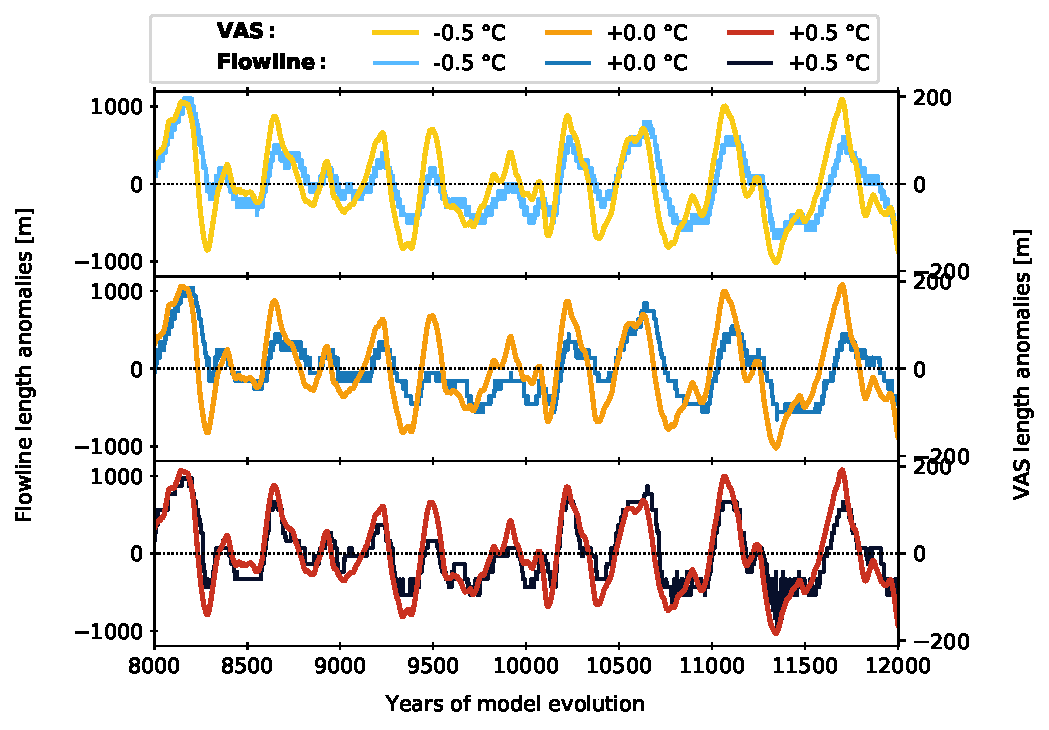
\includegraphics[width=\textwidth]{../plots/final_plots/random_length/Hintereisferner.pdf}
            \end{subfigure}
            \hfill
            \begin{subfigure}[b]{0.48\textwidth}
              \caption{RGI60-11.00106 - Pasterze}
              \label{fig:random_length:pasterze}
              \centering
              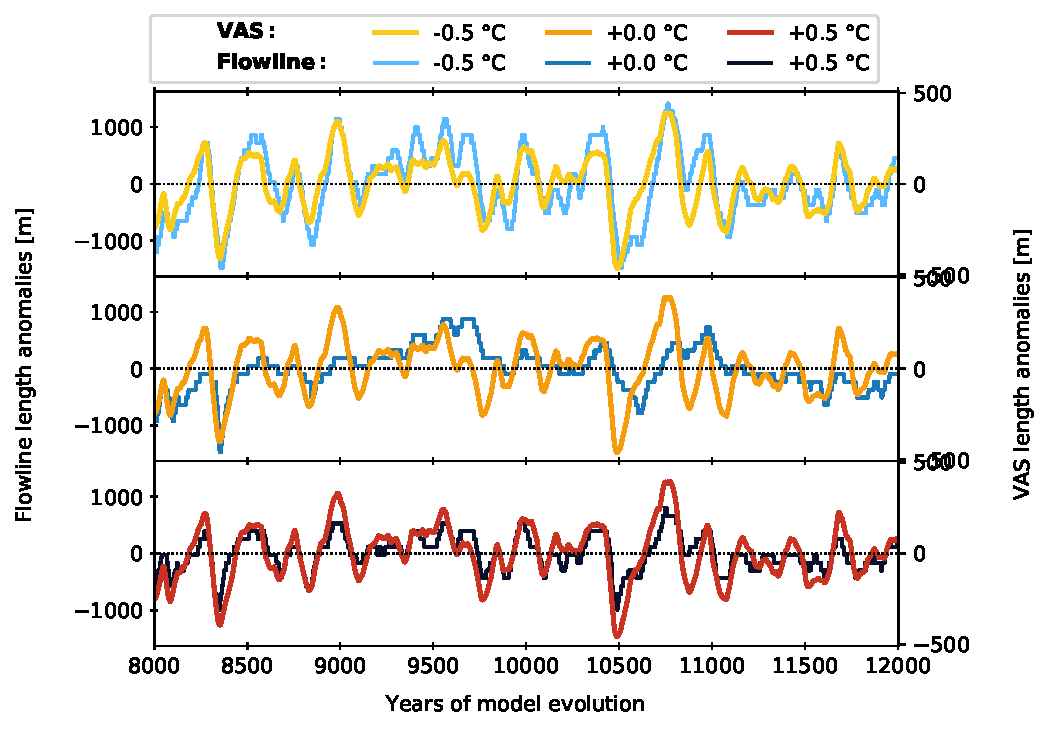
\includegraphics[width=\textwidth]{../plots/final_plots/random_length/Pasterze.pdf}
            \end{subfigure}
            \begin{subfigure}[b]{0.48\textwidth}
              \caption{RGI60-11.03643 - Mer de Glace}
              \label{fig:random_length:mer_de_glace}
              \centering
              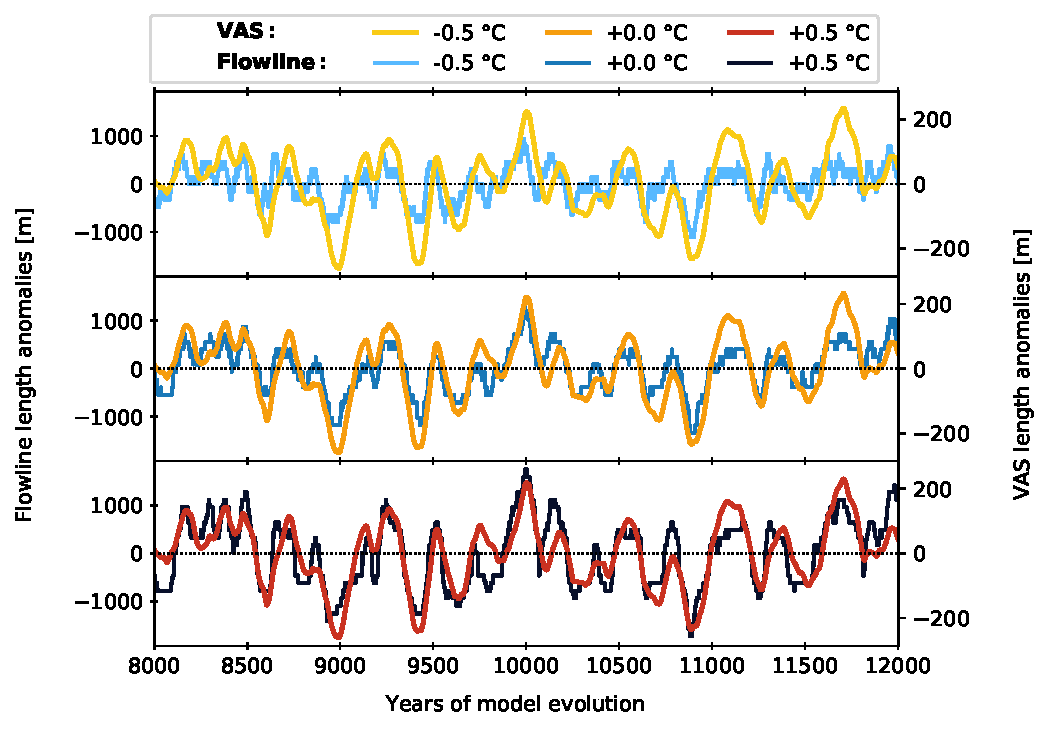
\includegraphics[width=\textwidth]{../plots/final_plots/random_length/Mer_de_Glace.pdf}
            \end{subfigure}
            \hfill
            \begin{subfigure}[b]{0.48\textwidth}
              \caption{RGI60-11.03638 - d'Argentière}
              \label{fig:random_length:glacier_d_argentiere}
              \centering
              \includegraphics[width=\textwidth]{../plots/final_plots/random_length/Glacier_d'Argentière.pdf}
            \end{subfigure}
            \begin{subfigure}[b]{0.48\textwidth}
              \caption{RGI60-11.01450 - Großer Aletschgletscher}
              \label{fig:random_length:großer_aletschgletscher}
              \centering
              \includegraphics[width=\textwidth]{../plots/final_plots/random_length/Großer_Aletschgletscher.pdf}
            \end{subfigure}
            \hfill
            \begin{subfigure}[b]{0.48\textwidth}
              \caption{RGI60-11.01238 - Rhonegletscher}
              \label{fig:random_length:rhonegletscher}
              \centering
              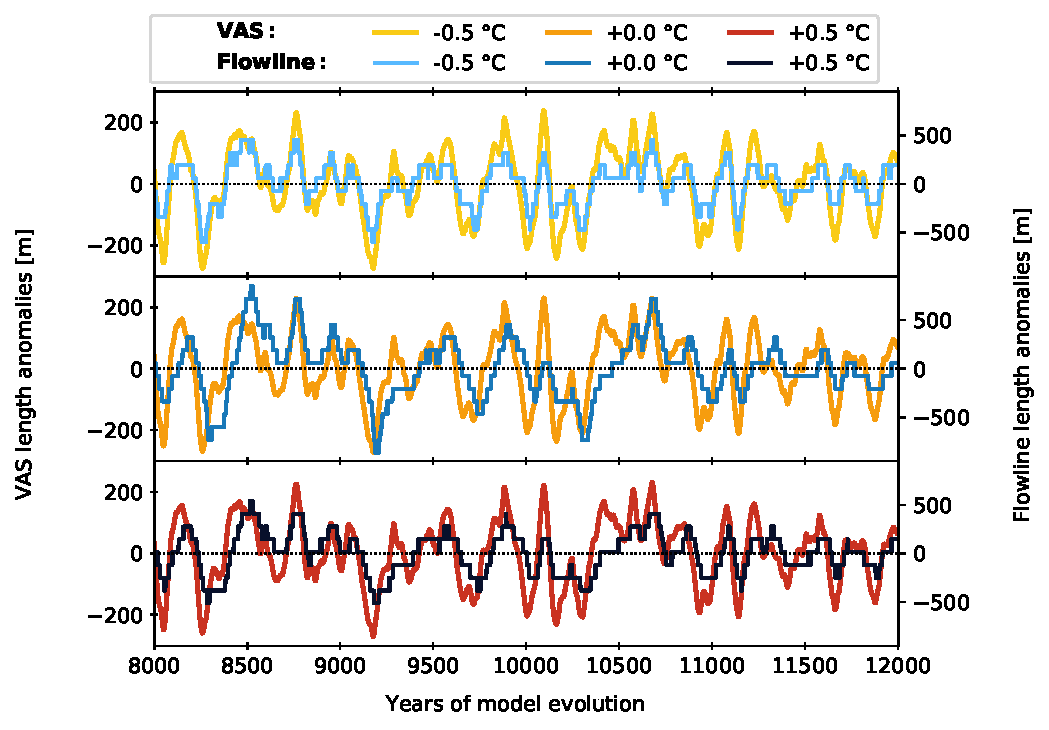
\includegraphics[width=\textwidth]{../plots/final_plots/random_length/Rhonegletscher.pdf}
            \end{subfigure}

            \caption{Length anomalies from to the respective average (equilibrium) value. The climate scenarios are based on a randomized equilibrium climate, with different temperature biases. Light blue, dark blue and ultramarine lines represent the flowline model, while yellow, orange and red lines represent the \vas{} model, with a temperature bias of \SI{-.5}{\celsius}, \SI{0}{\celsius} and \SI{+.5}{\celsius}, respectively. Note the differences in y-axis scales.}
            \label{fig:random_length} 
          \end{figure}

        Figure~\ref{fig:random_length} shows the length anomalies with respect to the equilibrium value for the arbitrarily chosen period between 8000 and 12\,000 years. This allows to formulate some first qualitative conclusions. The overlaid length changes seem to be in good agreement between the \vas{} and the flowline model. While correlations may be high, the difference in absolute length fluctuations is already apparent by looking at the y-scales (left for the flowline model and right for the \vas{} model). While the length changes estimated by the \vas{} model are all in the order of \SI{\pm200}{\meter} (except \SI{\pm500}{\meter} for the Pasterze, see Figure~\ref{fig:random_length:pasterze}), the flowline model predicts fluctuations between \SI{\pm500}{\meter} for the Rhonegletscher (Figure~\ref{fig:random_length:rhonegletscher}) and \SI{\pm2500}{\meter} for the Aletschgletscher (Figure~\ref{fig:random_length:großer_aletschgletscher}). Furthermore, different sizes of the same glacier show similar but noticeable different length fluctuation under the flowline model, while there seems to be little to no differences under the \vas{} model. However, these first findings are only based on the visual inspection of a temporally limited subsample and are further investigated and quantified in the following sections.

        
    
    % subsubsection length_anomalies_under_random_climate (end)
    
    \subsection{Power spectral density} % (fold)
    \label{sub:power_spectral_density_results}

      % PSD plots
      \begin{figure}[htp]
        \centering
        \begin{subfigure}[b]{0.48\textwidth}
          \caption{RGI60-11.00897 - Hintereisferner}
          \label{fig:psd:hintereisferner}
          \centering
          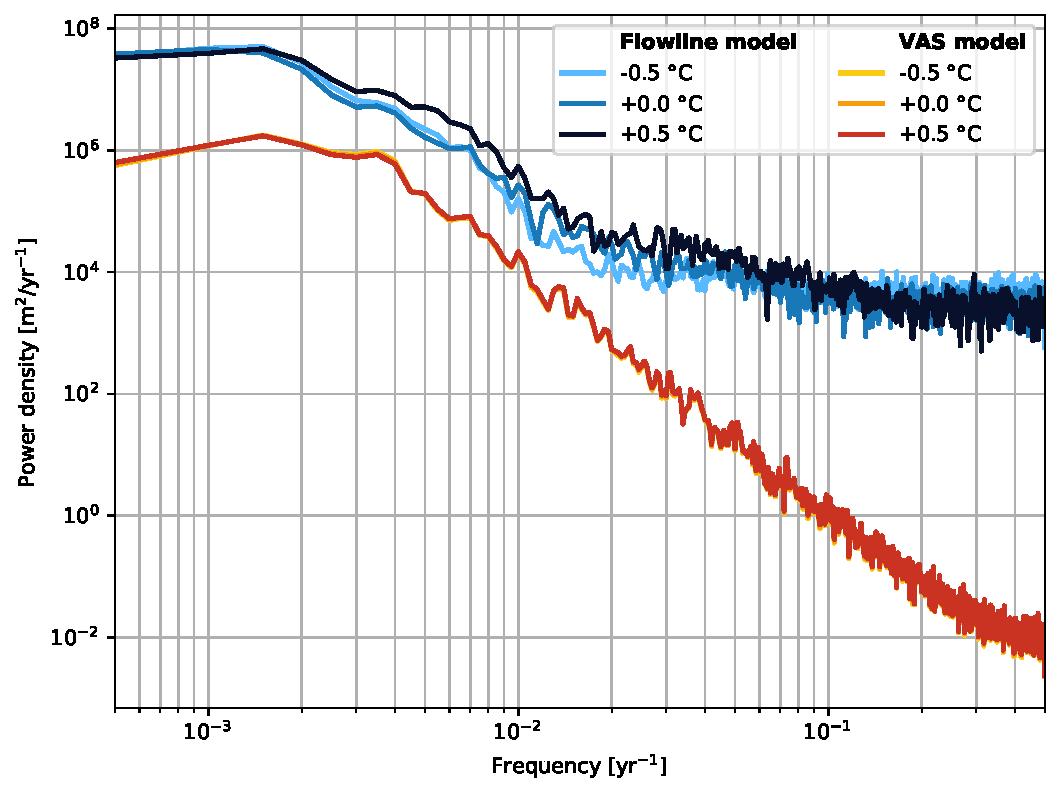
\includegraphics[width=\textwidth]{../plots/final_plots/psd/Hintereisferner.pdf}
        \end{subfigure}
        \hfill
        \begin{subfigure}[b]{0.48\textwidth}
          \caption{RGI60-11.00106 - Pasterze}
          \label{fig:psd:pasterze}
          \centering
          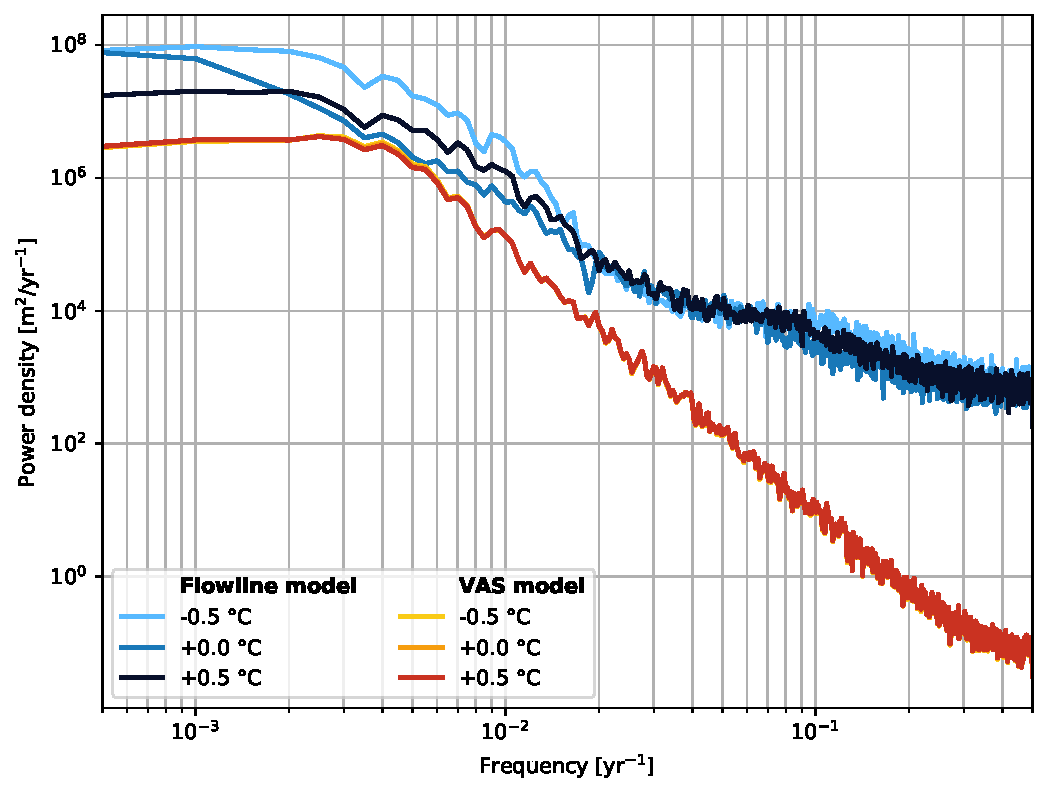
\includegraphics[width=\textwidth]{../plots/final_plots/psd/Pasterze.pdf}
        \end{subfigure}
        \begin{subfigure}[b]{0.48\textwidth}
          \caption{RGI60-11.03643 - Mer de Glace}
          \label{fig:psd:mer_de_glace}
          \centering
          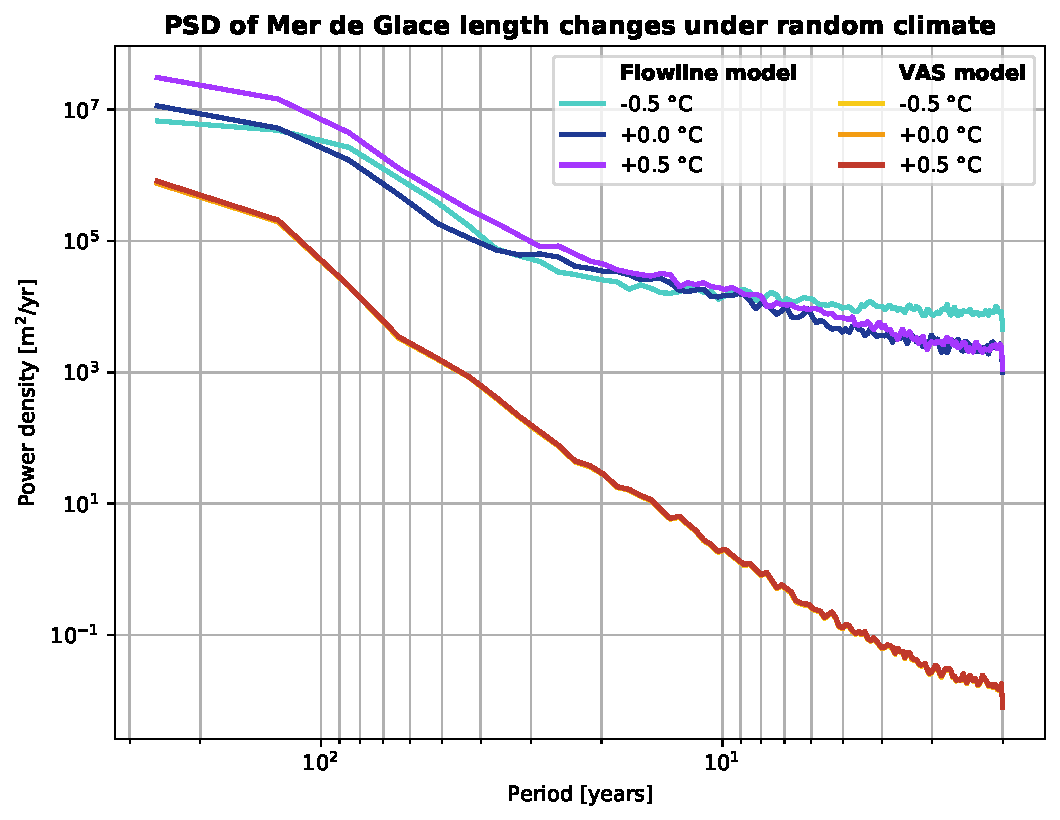
\includegraphics[width=\textwidth]{../plots/final_plots/psd/Mer_de_Glace.pdf}
        \end{subfigure}
        \hfill
        \begin{subfigure}[b]{0.48\textwidth}
          \caption{RGI60-11.03638 - d'Argentière}
          \label{fig:psd:glacier_d_argentiere}
          \centering
          \includegraphics[width=\textwidth]{../plots/final_plots/psd/Glacier_d'Argentière.pdf}
        \end{subfigure}
        \begin{subfigure}[b]{0.48\textwidth}
          \caption{RGI60-11.01450 - Großer Aletschgletscher}
          \label{fig:psd:großer_aletschgletscher}
          \centering
          \includegraphics[width=\textwidth]{../plots/final_plots/psd/Großer_Aletschgletscher.pdf}
        \end{subfigure}
        \hfill
        \begin{subfigure}[b]{0.48\textwidth}
          \caption{RGI60-11.01238 - Rhonegletscher}
          \label{fig:psd:rhonegletscher}
          \centering
          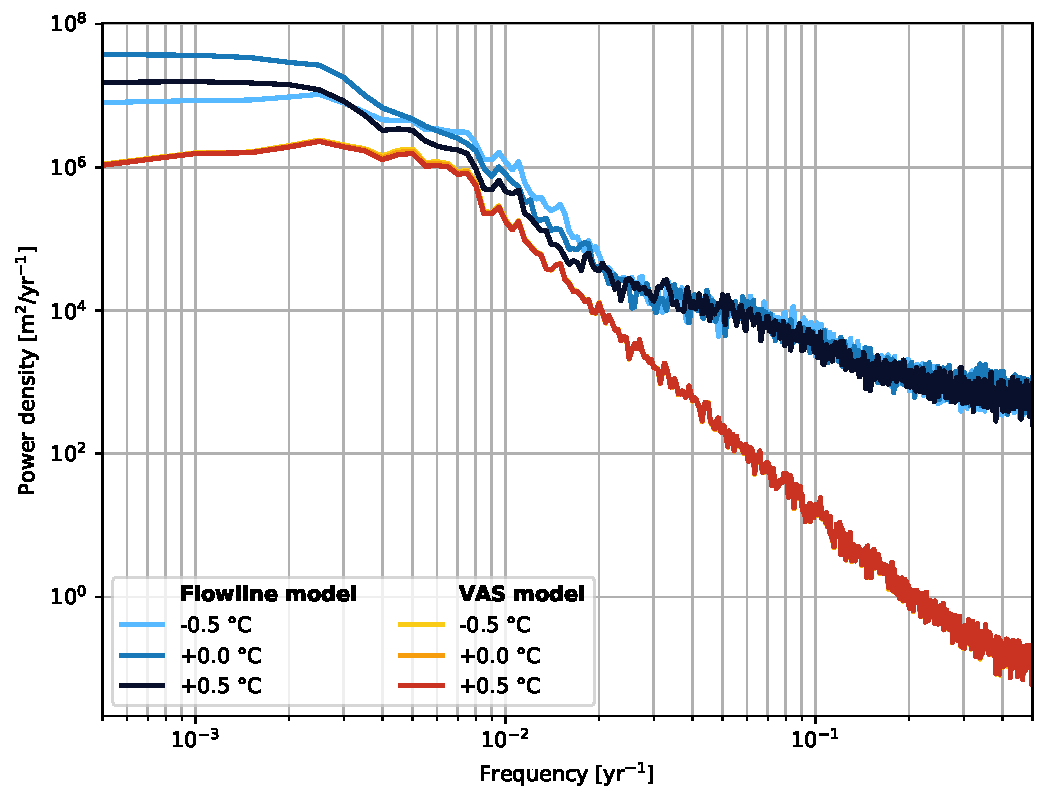
\includegraphics[width=\textwidth]{../plots/final_plots/psd/Rhonegletscher.pdf}
        \end{subfigure}

        \caption{Power spectral density of modeled glacier length for different alpine glaciers. Different lines represent different combinations of evolution models and climate scenarios. The climate scenarios are based on a randomized equilibrium climate, with different temperature biases. Light blue, dark blue and ultramarine lines represent the flowline model, while yellow, orange and red lines represent the \vas{} model, with a temperature bias of \SI{-.5}{\celsius}, \SI{0}{\celsius} and \SI{+.5}{\celsius}, respectively. Note the differences in y-axis scales.}
        \label{fig:psd}
      \end{figure}

      % intro and general
      % low pass filter
      Glaciers act as low-pass filters for the natural climate variability. A low pass filter passes lower frequencies while attenuating higher frequencies, which results in a characteristic PSD curve. Figure~\ref{fig:psd} shows the PSD of glacier lengths for the six glaciers mentioned above. The power density stays in a constant range for frequencies up to \SI{3e-3}{\per\year} (corresponding to signals with a period of over 300 years) before decreasing with increasing frequency. This makes intuitive sense, since changes in glacier length are mainly driven by long term climatic trends and less by inter-annual variabilities in the climatic forcing. A single year with low temperatures and strong (cold season) precipitation has less impact on the glacier size than a decade of slightly above-average temperatures.
      % higher power density of flowline model
      While the overall shape of the PSDs are similar for the \vas{} model and the flowline model, there are some key differences. As seen before, the length changes estimated by the \vas{} model are smaller compared to the flowline model. Hence, the overall power of the flowline model is higher across all frequencies. In agreement with the symmetric behavior discussed before, the PSDs of the \vas{} model are practically identical for different sizes of the same glacier. The PSDs based on the flowline length are less coherent between different sizes of the same glacier, whereby there is no discernible relation between shape of PSD and glacier size.
      % power density for high frequencies
      Additionally, the flowline model shows a rather constant power density for lower frequencies. This is due to the discrete changes in glacier length of the flowline model, whose resolution depends on the grid size (\SI{100}{\meter} in this case). The \vas{} model length is a continuous variable, resulting in a constantly decreasing power density.
      % slope?
      While the absolute values are different, the slope of the PSDs are almost identical between \vas{} and flowline model for medium frequencies up to about \SI{3e-2}{\per\year} (corresponding to signals with a period of over 30 years). This indicates that the breakdown of energy from larger to smaller scales happens at similar rates for both models (cf. the energy cascade for turbulent flows, e.g., \cite{Wyngaard2010}).
    
    % subsection power_spectral_density_results (end)

    \subsection{Autocorrelation function} % (fold)
    \label{sub:autocorrelation_function_results}

      % ACF figure
      \begin{figure}[htp]
        \centering
        
        \begin{subfigure}[b]{0.48\textwidth}
          \caption{RGI60-11.00897 - Hintereisferner}
          \label{fig:acf:hintereisferner}
          \centering
          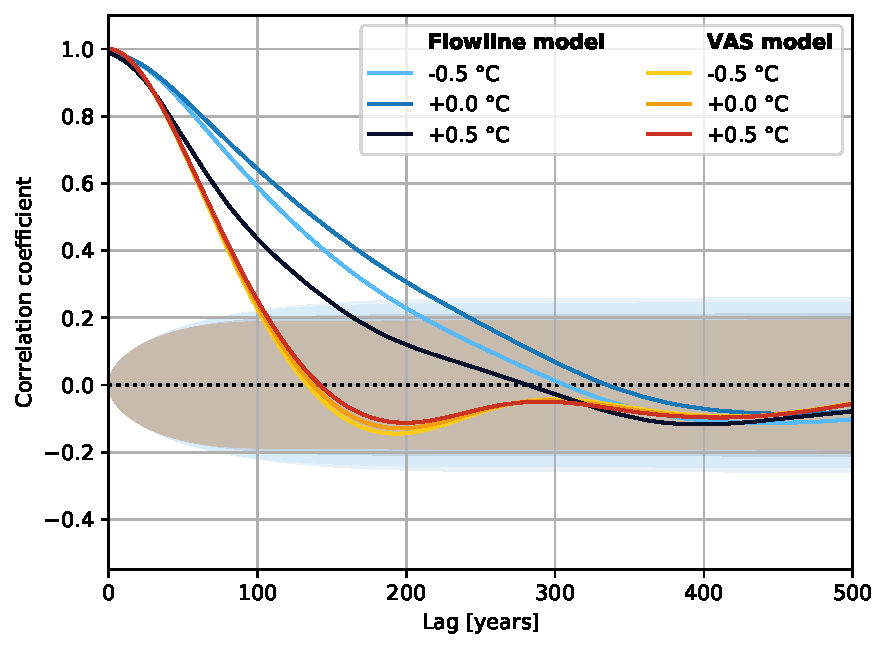
\includegraphics[width=\textwidth]{../plots/final_plots/acf/Hintereisferner.pdf}
        \end{subfigure}
        \hfill
        \begin{subfigure}[b]{0.48\textwidth}
          \caption{RGI60-11.00106 - Pasterze}
          \label{fig:acf:pasterze}
          \centering
          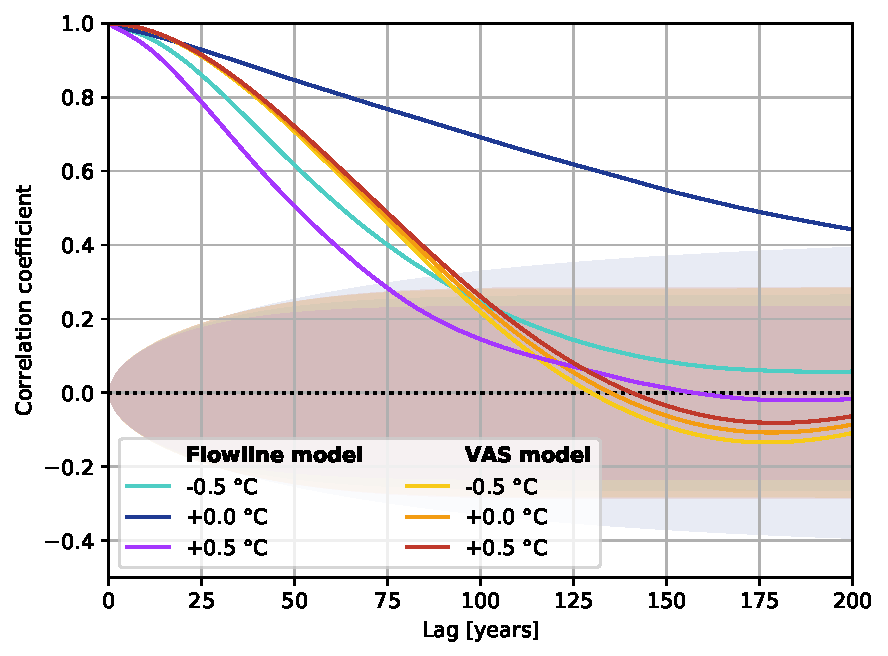
\includegraphics[width=\textwidth]{../plots/final_plots/acf/Pasterze.pdf}
        \end{subfigure}

        \begin{subfigure}[b]{0.48\textwidth}
          \caption{RGI60-11.03643 - Mer de Glace}
          \label{fig:acf:mer_de_glace}
          \centering
          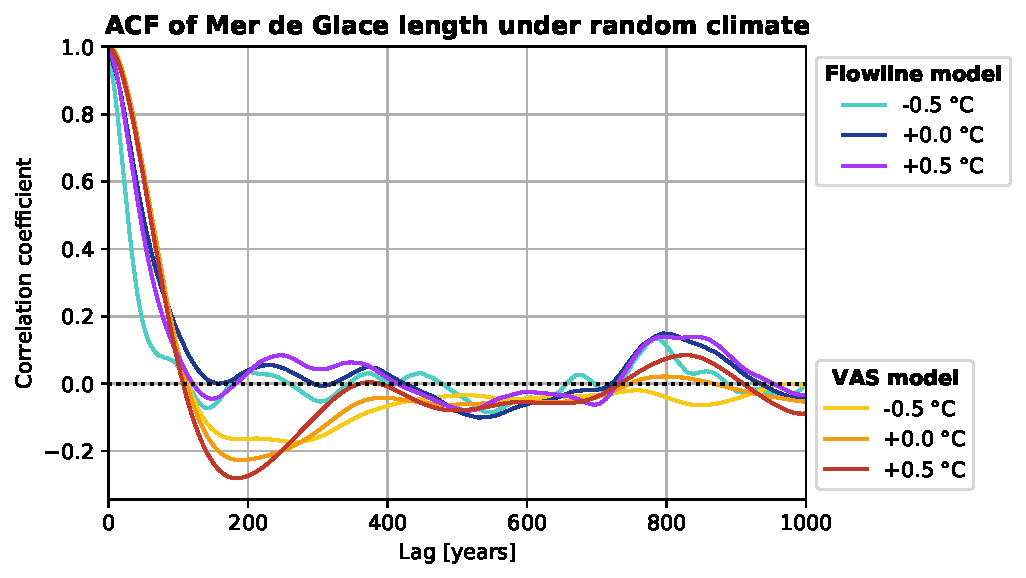
\includegraphics[width=\textwidth]{../plots/final_plots/acf/Mer_de_Glace.pdf}
        \end{subfigure}
        \hfill
        \begin{subfigure}[b]{0.48\textwidth}
          \caption{RGI60-11.03638 - d'Argentière}
          \label{fig:acf:glacier_d_argentiere}
          \centering
          \includegraphics[width=\textwidth]{../plots/final_plots/acf/Glacier_d'Argentière.pdf}
        \end{subfigure}

        \begin{subfigure}[b]{0.48\textwidth}
          \caption{RGI60-11.01450 - Großer Aletschgletscher}
          \label{fig:acf:großer_aletschgletscher}
          \centering
          \includegraphics[width=\textwidth]{../plots/final_plots/acf/Großer_Aletschgletscher.pdf}
        \end{subfigure}
        \hfill
        \begin{subfigure}[b]{0.48\textwidth}
          \caption{RGI60-11.01238 - Rhonegletscher}
          \label{fig:acf:rhonegletscher}
          \centering
          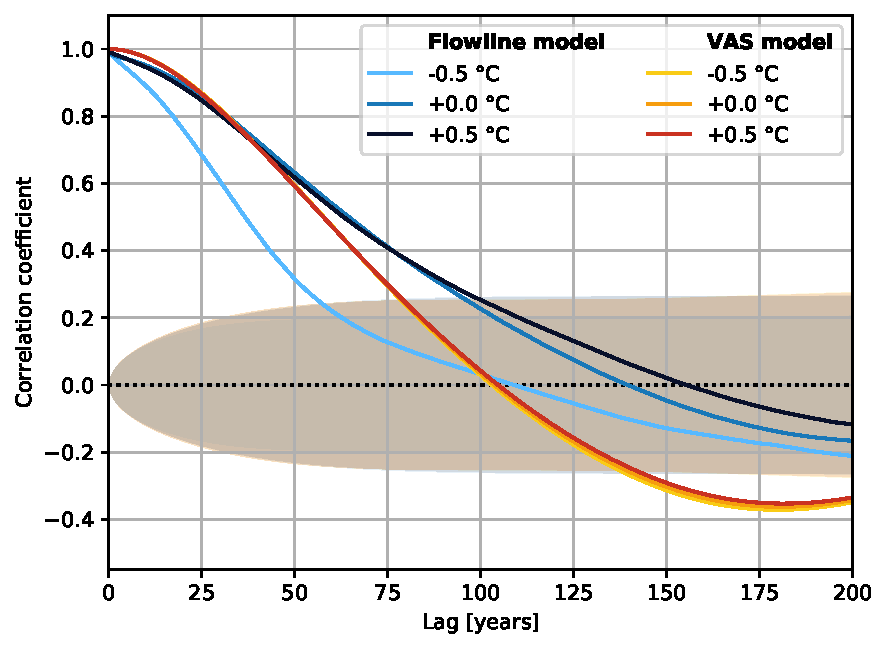
\includegraphics[width=\textwidth]{../plots/final_plots/acf/Rhonegletscher.pdf}
        \end{subfigure}

        \caption{Autocorrelation function of modeled length for lag times between zero and 200 years. Different lines represent different combinations of evolution model and climate scenario.
        The random climate scenario is based on an equilibrium climate, with different temperature biases.
        Light blue, dark blue and ultramarine represent the flowline model, while yellow, orange and red lines represent the \vas{} model, with a temperature bias of \SI{-.5}{\celsius}, \SI{0}{\celsius} and \SI{+.5}{\celsius}, respectively.
        The \SI{99}{\percent} confidence intervals are shaded in the corresponding colors.}
        \label{fig:acf}
      \end{figure}
      % End ACF figure

      Figure~\ref{fig:acf} shows the autocorrelation function (ACF) of modeled glacier length for lag times up to 200 years. A general observation about the ACF can be made for both models, all glaciers and climate scenarios: the correlation is high for the first few lag times, before it decreases exponentially. This points at an autoregressive (AR) term and a moving-average (MA) term in the data. An autoregressive-moving-average model (ARMA) predicts future values of a random variable based on a linear combination of the past values and past error terms of said variable. This makes intuitive sense for glaciers, since the past and current glacier size and the difference to the equilibrium value have a direct influence on next years glacier size. A more detailed discussion of a potential ARMA model is provided at the end of this section.

      Same as for the PSDs, the ACFs for the \vas{} length signals are almost identical between different sizes of the same glacier, indicating that the glacier size has little to no effect on the transient behavior of the model. The \vas{} model represents the glacier as a simple cuboid without any additional information about the glacier shape. The absolute dimensions of that cuboid seem to have less of an effect on the ACF than other parameters, which differ from glacier to glacier. Some glaciers, like the Glacier d'Argentière and the Aletschgletscher show statistically significant negative correlations for higher lag terms between 80 and 250 years, while the others show very little to no significant negative correlation for higher lag times. However, no apparent relation between the strength of negative correlations for later lag times and any other glacier parameter, like the average slope or the model-internal lag times, was found.
      The average slope is the only additional geometric information of the \vas{} model, even if it is implemented only indirectly. It is computed as the relation between elevation range (extracted from the DEM) and glacier length (scaled from the RGI area), and thereby somewhat independent of the other scaled glacier geometries.
      However, it affects the temporal evolution, since changes in terminus elevation---and thereby changes in specific mass balance---are linearly related to changes in glacier length. This can be seen in the ACF plots, which vary from glacier to glacier but not between different sizes of the same glacier.  However, their is no obvious pattern when comparing the ACF to the average slope.
    
      The flowline model is able to represent different glacier geometries and grasp individual responses under different equilibrium climates, which can be seen in the vastly different ACFs. They differ from glacier to glacier, but also for different sizes of the same glacier. However, there are again no discernible patterns, which confirms the notion that the flowline model is capable of simulating each glacier's individual response. The autocorrelation of the flowline model is generally stronger than for the \vas{} runs for most glaciers and most temperature biases, even though not for all. The following list points to some particular observations:
      \begin{itemize}
        \item for Hintereisferner (Figure~\ref{fig:acf:hintereisferner}) the ACFs of the flowline model show higher correlations than for the \vas{} model, while for Mer de Glace (Figure~\ref{fig:acf:mer_de_glace}) and Großer Aletschgletscher (Figure~\ref{fig:acf:großer_aletschgletscher}) the flowline model ACFs show equal or lower correlations for lag time up to around fifty years;
        \item the flowline model of the Pasterze (Figure~\ref{fig:acf:pasterze}) shows a strong autocorrelation under the equilibrium climate, i.e., for its medium size, ($r>0.6$ for lags times up to one-hundred years and statistically significant up until a lag time of 243 years), while under a warmer and colder equilibrium climate (\SI{\pm0.5}{\celsius}) the autocorrelation of all lag times is comparable to the \vas{} model;
        \item similarly, the flowline model of the Glacier d'Argentière (Figure~\ref{fig:acf:glacier_d_argentiere}) shows a strong autocorrelation under the warmer equilibrium climate (\SI{+0.5}{\celsius}), while the autocorrelation under the other two climate scenarios is even lower than the ACF of the \vas{} model.
      \end{itemize}
      The only observation made for all glaciers, it that the \vas{} model shows a stronger or equal autocorrelation for shorter lag time (i.e., less than about twenty years) than the flowline model. This is true even for glaciers, where the autocorrelation of the flowline mode is generally stronger than for the \vas{} model (e.g., Hintereisferner).

      % PACF figure
      \begin{figure}[htp]
        \centering
        
        \begin{subfigure}[b]{0.48\textwidth}
          \caption{RGI60-11.00897 - Hintereisferner}
          \label{fig:pacf:hintereisferner}
          \centering
          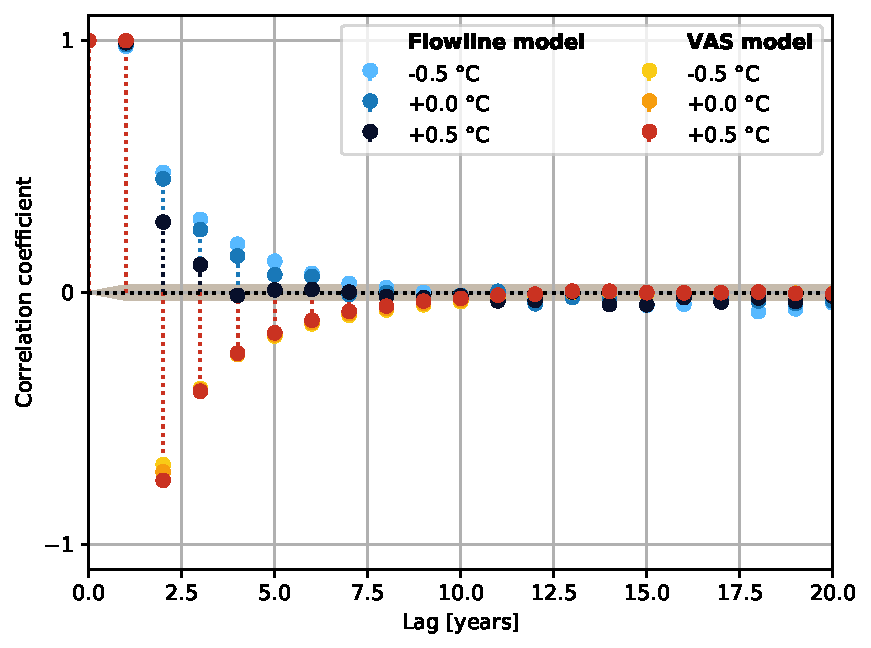
\includegraphics[width=\textwidth]{../plots/final_plots/pacf/Hintereisferner.pdf}
        \end{subfigure}
        \hfill
        \begin{subfigure}[b]{0.48\textwidth}
          \caption{RGI60-11.00106 - Pasterze}
          \label{fig:pacf:pasterze}
          \centering
          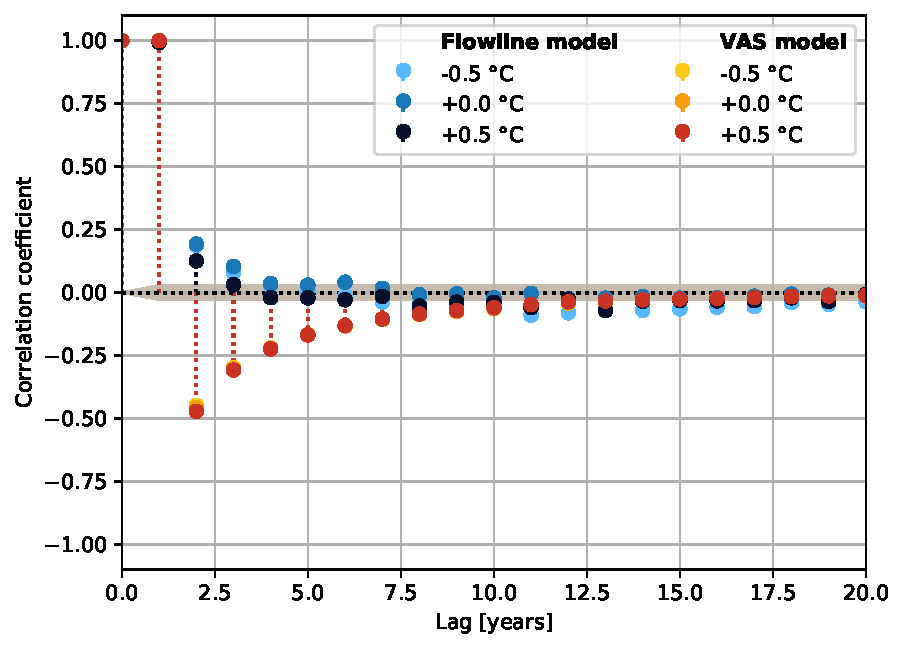
\includegraphics[width=\textwidth]{../plots/final_plots/pacf/Pasterze.pdf}
        \end{subfigure}

        \begin{subfigure}[b]{0.48\textwidth}
          \caption{RGI60-11.03643 - Mer de Glace}
          \label{fig:pacf:mer_de_glace}
          \centering
          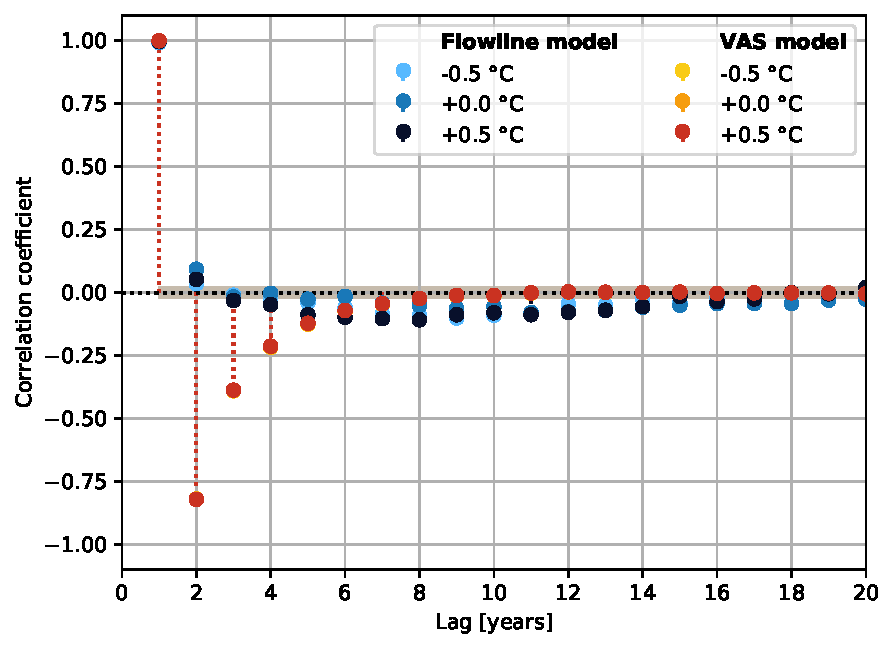
\includegraphics[width=\textwidth]{../plots/final_plots/pacf/Mer_de_Glace.pdf}
        \end{subfigure}
        \hfill
        \begin{subfigure}[b]{0.48\textwidth}
          \caption{RGI60-11.03638 - d'Argentière}
          \label{fig:pacf:glacier_d_argentiere}
          \centering
          \includegraphics[width=\textwidth]{../plots/final_plots/pacf/Glacier_d'Argentière.pdf}
        \end{subfigure}

        \begin{subfigure}[b]{0.48\textwidth}
          \caption{RGI60-11.01450 - Großer Aletschgletscher}
          \label{fig:pacf:großer_aletschgletscher}
          \centering
          \includegraphics[width=\textwidth]{../plots/final_plots/pacf/Großer_Aletschgletscher.pdf}
        \end{subfigure}
        \hfill
        \begin{subfigure}[b]{0.48\textwidth}
          \caption{RGI60-11.01238 - Rhonegletscher}
          \label{fig:pacf:rhonegletscher}
          \centering
          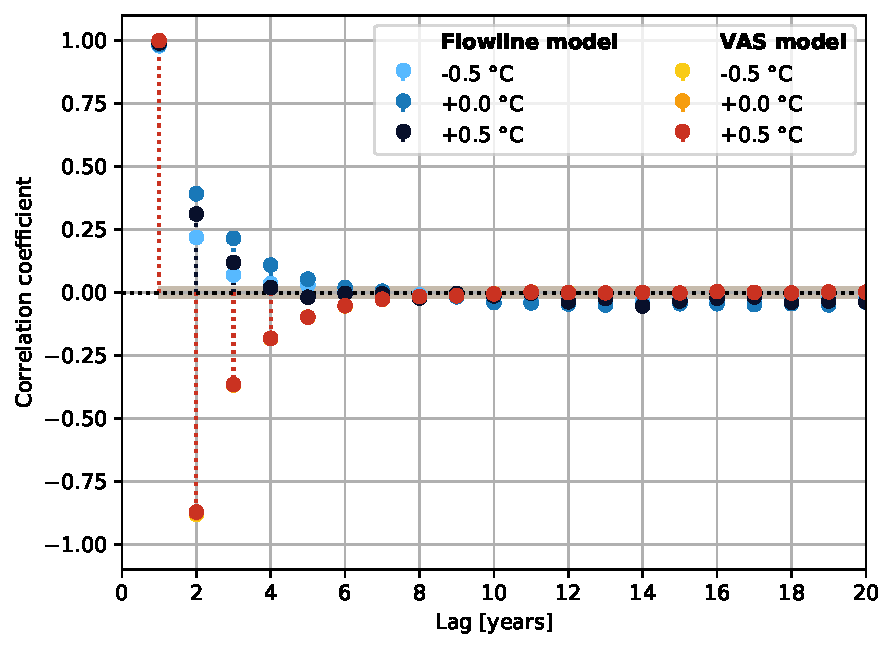
\includegraphics[width=\textwidth]{../plots/final_plots/pacf/Rhonegletscher.pdf}
        \end{subfigure}

        \caption{Partial autocorrelation function of modeled length for lag times between zero and 200 years. Different lines represent different combinations of evolution model and climate scenario.
        The random climate scenario is based on an equilibrium climate, with different temperature biases.
        Light blue, dark blue and ultramarine dots represent the flowline model, while yellow, orange and red dots represent the \vas{} model, with a temperature bias of \SI{-.5}{\celsius}, \SI{0}{\celsius} and \SI{+.5}{\celsius}, respectively.
        The \SI{99}{\percent} confidence intervals are shaded in the corresponding colors.}
        \label{fig:pacf}
      \end{figure}
      % End PACF figure

      Figure~\ref{fig:pacf} shows the partial autocorrelation function (PACF) of modeled glacier length for lag times up to twenty years. The PACF measures only the direct influences from one point in time to the following, eliminating the effects of all shorter lag times. This is an important additional measure, since strong correlations for short lag times influences the correlation of all following lag terms. Consider, for example, an exponentially decaying signal, which halves its value with each time step $\Phi(t) = 0.5 \Phi(t-1)$, will have an autocorrelation of 0.5 for lag 1, 0.25 for lag 2, 0.125 for lag 3, and so on. Depending on the sample size these values will be statistically significant. However, in this example only the previous value $\Phi(t-1)$ has a direct effect on the current one $\Phi(t)$, since only one lag term is included in the definition of the signal. The PACF will only show a significant correlation at lag one, i.e., defining an AR(1) process.

      All the PACFs of the \vas{} model lengths (left panels of Figure~\ref{fig:pacf}) show a strong positive correlation for lag times of 1 year, followed by a strong negative correlation which then slowly increases towards zero. Correlations for lag times ten and greater are not, or only marginally, significant. Again, there are no discernible differences between different sizes of the same glacier and very little differences from one glacier to another. The PACFs for the flowline model lengths show the same high correlation for the lag time of one year, before decreasing towards zero. The decrease towards statistical insignificant correlations happens quite fast for most glaciers. Only Mer de Glace (Figure~\ref{fig:pacf:mer_de_glace}) and Glacier d'Argentière (Figure~\ref{fig:pacf:glacier_d_argentiere}), both for the warmer climate, and Rhonegletscher (Figure~\ref{fig:pacf:rhonegletscher}), for the equilibrium climate, show significant correlations for lag times greater than three years. For higher lag times between ten and twenty years there are some negative correlations, even though they are only marginally significant. This indicates that the length of the previous year has a strong direct influence on the current length (almost 1:1), while length of two or more years back has only a weak direct (for the flowline model) or even an inverse influence (for the \vas model). Those results mainly from the mathematical derivation of the PACF and has hence little physical meaning.

      The number of statistically significant terms of the PACF informs on the order $p$ for the AR($p$) model. The order specifies the of number lag terms that are considered. Analogously, the order $q$ for the MA($q$) model can be estimated from the number of significant terms of the ACF. By this definition, the \vas{} model could be represented by an ARMA(9, 70) model, and the flowline model by an ARMA(3, 140). Hereby, the orders are taken as average over all glaciers and climate scenarios (see Appendix~\ref{appendix_B} for details). While an AR model with nine lag terms would be big but still feasible, a MA model with over one-hundred lag terms is neither practicable nor does it make sense. Especially, since \citet{Roe2014} use an ARMA(3,3) model to produce comparable results to a flowline model. It is not the intent of this work to investigate the relation between a glacier's geometry and its ACF, neither to fit an ARMA model to the data. However, it is most notable that the flowline model behaves differently not only for different glaciers, but also for different sizes of the same glacier. The \textit{one size fits all} approach of the \vas{} model produces more homogeneous results, the ACFs and PACFs are mostly independent of a glacier's size.

    % subsection autocorrelation_function_results (end)

  % section autocorrelation_fand_power_spectral_density_results (end)

  \section{Regional runs with all Alpine glaciers} % (fold)
  \label{sec:regional_runs_with_all_alpine_glaciers_results}

    \Vas{} applied to single glaciers gives only an order of magnitude estimation, since the scaling constant $c$ is a globally averaged value. A potential relative error in $c$ will be directly transfered to any volume estimation \citep{Bahr2015}. Hence, \vas{} should not be applied to individual glaciers, but only to populations of glaciers, where the scaling approach shows its strength: the law of large number assures a reasonable estimation of the collective glacier ice volume, since random errors will be canceled out by each other \citep{Bahr2015}.
    The first regional simulation over Alpine glaciers shown in this section, compares the behavior of the \vas{} model to the flowline model under different climate scenarios (analogous to the single glacier test case, see Section~\ref{sec:single_glacier_test_case_results}).

    \subsection{Experimental setup} % (fold)
    \label{sub:experimental_setup_regional_run}

        The experimental setup is analogous to the single glacier test case, again comparing the \vas{} model to the flowline model, with some minor modifications. To best reflect the regional glacial evolution, the default OGGM \hyperref[ssub:mb_calib]{mass balance calibration} is used (see Section~\ref{sub:temperature_index_model}). This means, each evolution model uses its own \tstar{} reference table (which may result in different \tstar{} for the same glacier depending on the evolution model). The mass balance residual is again omitted ($\beta^* = 0$), since this experiment intends to investigate the model behavior rather than absolute real-world values.
        Both evolution models run with the \lstinline`ConstantMassBalance` model and the \lstinline`RandomMassBalance` model, for 1000 years each. The mass balance models are initialized with \lstinline`y0` = \tstar{} and run with the same three different temperature biases as before (\SI{0}{\celsius}, \SI{-0.5}{\celsius}, \SI{+0.5}{\celsius}).
    
    % subsection experimental_setup (end)

    \subsection{Results} % (fold)
    \label{sub:results_regional_run}

        % Figure HISTALP run
        \begin{figure}[t!]
          \centering
          \begin{subfigure}[b]{0.48\textwidth}
            \caption{\Vas{} model, relative glacier volume}
            \label{fig:histalp_commitment:volume_norm_const}
            \centering
            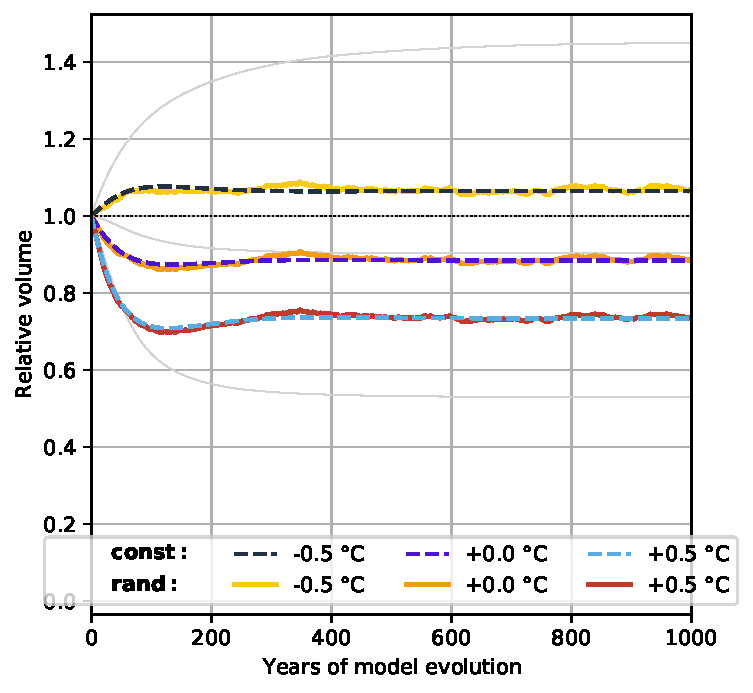
\includegraphics[width=\textwidth]{../plots/final_plots/time_series/histalp_commitment/volume_norm_vas.pdf}
          \end{subfigure}
          \hfill
          \begin{subfigure}[b]{0.48\textwidth}
            \caption{Flowline model, relative glacier volume}
            \label{fig:histalp_commitment:volume_norm_random}
            \centering
            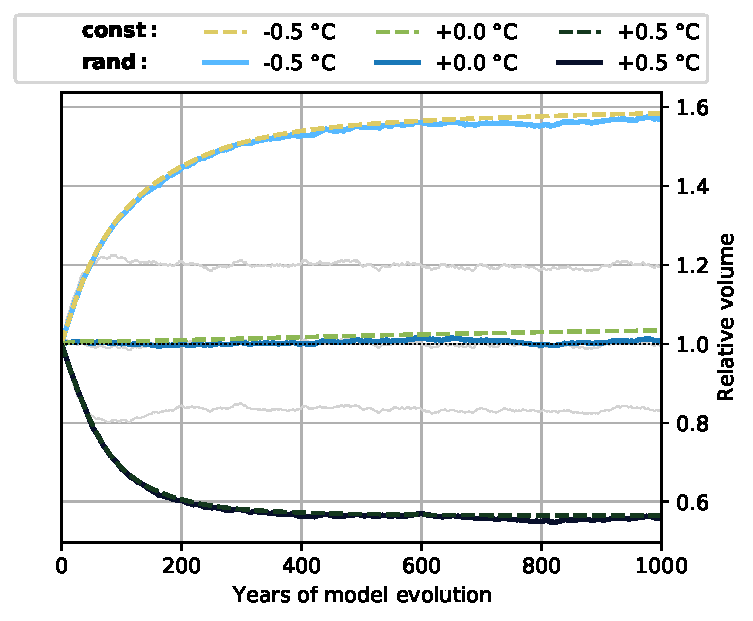
\includegraphics[width=\textwidth]{../plots/final_plots/time_series/histalp_commitment/volume_norm_fl.pdf}
          \end{subfigure}
          % Absolute volume
          \begin{subfigure}[b]{0.48\textwidth}
            \caption{\Vas{} model, absolute glacier volume}
            \label{fig:histalp_commitment:volume_abs_const}
            \centering
            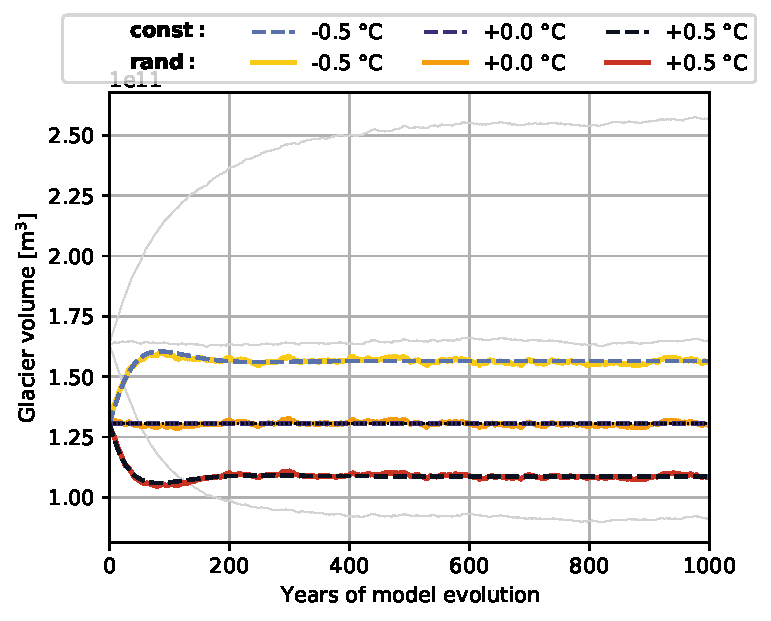
\includegraphics[width=\textwidth]{../plots/final_plots/time_series/histalp_commitment/volume_abs_vas.pdf}
          \end{subfigure}
          \hfill
          \begin{subfigure}[b]{0.48\textwidth}
            \caption{Flowline model, absolute glacier volume}
            \label{fig:histalp_commitment:volume_abs_random}
            \centering
            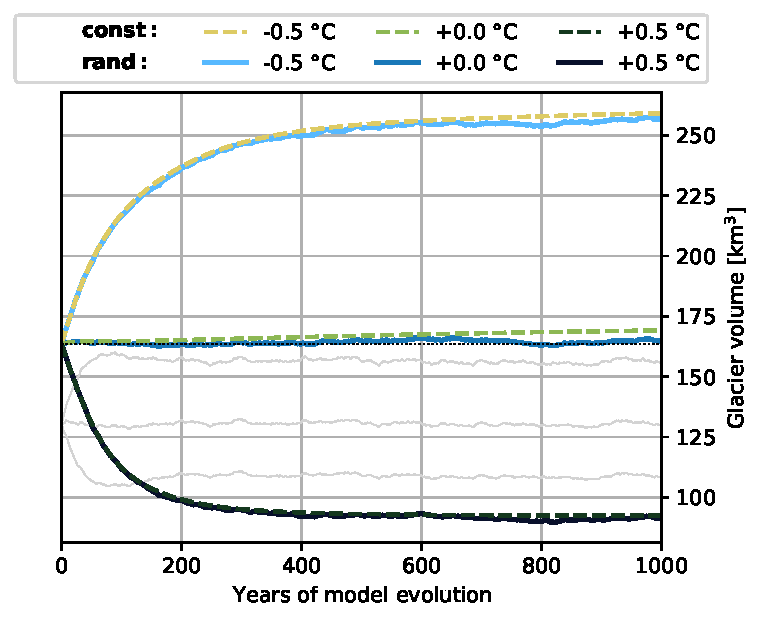
\includegraphics[width=\textwidth]{../plots/final_plots/time_series/histalp_commitment/volume_abs_fl.pdf}
          \end{subfigure}
          
          \caption{Time series of relative ice volume normalized with the initial values (upper panels) and absolute ice volume (lower panels), for all glaciers in the HISTALP domain. The left panels show the result of the \vas{} model, the right panels show the results of the flowline model. Solid lines represent the random climate scenarios, while dashed lines represent the constant climate scenarios. All climate scenarios are based on an equilibrium climate. The applied temperature biases of \SI{-.5}{\celsius}, \SI{0}{\celsius} and \SI{+.5}{\celsius} are color coded, see legend for details. Light gray lines represent the volume evolutions of the other model, to facilitate comparisons.}
          \label{fig:histalp_commitment}
        \end{figure}
        % End Figure HISTALP run

        Figure~\ref{fig:histalp_commitment} shows the temporal evolution of aggregate glacier ice volume of all Alpine glaciers for the \vas{} model (left panel) and the flowline model (right panel) with three different equilibrium climates each. Both evolution models run for 1000 years with the \lstinline`ConstantMassBalance` model and the \lstinline`RandomMassBalance` model. The random climate with its year-to-year fluctuations is more physical than the completely constant climate. However, the resulting changes in glacier ice volume under both climate scenarios are almost identical. This makes intuitive sense, considering that glaciers act as natural low-pass filters for climatic variabilities (as established above, see Section~\ref{sub:power_spectral_density_results}). Short term climatic variabilities have little to no effect on the ice volume of a single glacier, much less on the aggregate ice volume of an entire region. Over the last 200 years of the simulations, the relative differences in aggregate ice volume between the constant and random climate scenario never exceed \SI{0.6}{\percent} for the \vas{} model and \SI{1.7}{\percent} for the flowline model. Only the \SI{0}{\celsius}-run of flowline model shows higher relative differences, with an average of \SI{2.0}{\percent} over the last 200 years, up to a maximum of \SI{2.7}{\percent}. While the total ice volume stays close to its initial value, it shows a slight increase over time. After an initially strong increase of \SI{1.6}{\percent} over the first fifty years and another fifty years of constant values, the volume grows almost linearly with about \SI{0.53}{\cubic\kilo\meter} per 100 years under the constant climate scenario. This results in a total volume change of \SI{5.6}{\cubic\kilo\meter} (\SI{+3.4}{\percent} of the initial value) after 1000 years of simulation. Under the random climate scenario, the total ice volume grows slower, most likely since the oscillations will reduce certain feedback loops. Hence, the following discussion is simplified by only considering the constant climate scenarios. 

        The \vas{} model estimates a total Alpine ice volume of \SI{156}{\cubic\kilo\meter} (\SI{+20}{\percent}), \SI{130}{\cubic\kilo\meter} (\SI{\pm{}0}{\percent}) and \SI{109}{\cubic\kilo\meter} (\SI{-17}{\percent}), while the flowline model estimates a total Alpine ice volume of \SI{259}{\cubic\kilo\meter} (\SI{+59}{\percent}), \SI{169}{\cubic\kilo\meter} (\SI{+3}{\percent}) and \SI{92}{\cubic\kilo\meter} (\SI{-44}{\percent}), after 1000 years of simulation under a temperature bias of \SI{-0.5}{\celsius}, \SI{0}{\celsius} and \SI{+0.5}{\celsius}, respectively. The \vas{} model estimate is much closer to the consensus estimate of \citet{Farinotti2019}, a detailed discussion is provided in Section~\ref{sec:relative_and_absolute_values_of_ice_volume_change}.

        All the general characteristics of the \vas{} model found for the Hintereisferner test case turn up again for the regional. The changes in ice volume estimated by the \vas{} scaling model are much smaller when compared to the flowline model, by a factor of \num{\approx 3.5}. The oscillatory behavior of the \vas{} model is still visible. The \vas{} model's response time scales to the step changes in climate are shorter that for the flowline model. The volume e-folding time scales of both models are comparable to the single glacier test case: $\tau_V = \SI{23}{\year}$ and $\tau_V = \SI{20}{\year}$ for the \vas{} model and $\tau_V = \SI{125}{\year}$ and $\tau_V = \SI{79}{\year}$ for the flowline model, for the negative and positive temperature perturbation, respectively. These values are highly influenced by the larger glaciers and serve only as a guidance level. The symmetric behavior of the \vas{} model is still reflected in the response times, but less so in the new equilibrium values.
        
        The next section explores the possibilities of tuning the \vas{} model via different parameters for the used scaling relations. This also provides a range of plausible results and serves as uncertainty estimation.

    % subsection results (end)

  % section regional_runs_with_all_alpine_glaciers_results (end)

  \section{Sensitivity experiments} % (fold)
  \label{sec:sensitivity_experiments_results}

    Before moving to the final experiments of projecting the future ice mass loss in the Alps and High Mountain Asia, it is necessary to determine the model's sensitivities. The following sensitivity analysis investigates the effects of the model-internal time scales and the scaling parameters on the model behavior. Both parameter sets are specific to the scaling model, since they determine the response time scaling as well as the volume/length and \vas{}. For consistency, the sensitivity experiments are performed on Hintereisferner (RGI60-11.00897) as a single glacier test case and on all Alpine glaciers inside the HISTALP domain. For simplicity, only the \lstinline`ConstantMassBalance` model with a temperature bias of \SI{+0.5}{\celsius} is used for all runs.

    \begin{tldrbox}[Sensitivity experiments]{tldr:sensitivity_experiments_results}
      \item The model-internal time scales control the damping ratio of the oscillation, longer time scales correspond to stronger overshoots.
      \item Halving the model-internal time scales leads to an almost asymptotic change in aggregate ice volume of the HISTALP domain, showing only negligible oscillations.
      \item Different scaling constants lead to a different initial ice volume and a different initial glacier length, which in turn affect the e-folding time scales.
      \item Changing the scaling constants has little to no effect on the normalized volume change and normalized equilibrium volume.
      \item Custom scaling constants and exponents increase the change in ice volume ever so slightly, but the results are still not comparable to the flowline model.
    \end{tldrbox}

    \subsection{Experimental setup} % (fold)
    \label{sub:experimental_setup_sensitivity}

        % Time scales
        The scaling model estimates glacial evolution via the implemented response time scaling. Response time scaling adjusts the yearly changes in length and area, in relation to the total possible changes, using the model-internal response time scales for length and area, $\tau_L$ and  $\tau_A$, respectively.
        The estimate for the model-internal time scales loosely follows \citet{Johannesson1989} (see Section~\ref{sub:glacier_evolution_model} and \ref{sub:glacier_evolution_model_implementation} for details). However, the model-internal time scales are good possible tuning parameters. The sensitivity experiments compare the model output for different time scales, modified by a linear factor $\tau_\text{sens.} = f \cdot \tau$. Hereby, the factor $f$ is only applied to $\tau_L$, since $\tau_A$ is a just linear function of $\tau_L$. Starting from the default value ($f=1$) as baseline, the effects of halved ($f=0.5$) and doubled ($f=2$) model-internal time scales are investigated.

        % Scaling parameters
        The other obvious choice for tuning parameters are the scaling exponents and scaling constants. The scaling constants for volume/length and \vas{}, $c_L$ and $c_A$, respectively, can be seen as random variables. The randomness stems from the statistically similar, but not identical, dimensionless parameters for length, area and volume  varying from glacier to glacier. Thanks to the law of large numbers, the global scaling constants $c_L = \SI{0.0180}{\kilo\meter^{3-q}}$ and $c_A = \SI{0.0340}{\kilo\meter^{3-2\gamma}}$ are a reasonable choice for a global ice volume estimation \citep{Bahr2015}. However, those parameters may be a bad fit for certain regions and therefore need calibration.
        While the scaling constants are not constant, the scaling exponents are. The \vas{} exponent was first derived as the slope of the linear regression of volume and area observations in log-log space \citep[e.g.,][]{Chen1990}. \citet{Bahr1997b} found that their values are fixed by the underlying physics and depend only on a single set of closure conditions. The closure conditions are in turn tightly bound by observations. Different common closures lead to the same results. Hence, it is strongly advised to use the global values of $q = 2.2$ and $\gamma = 1.375$  for the volume/length and \vas{}. Furthermore, even if different closure conditions could be justified, the area scaling exponent is bound $1.1\dot{6} \leq \gamma \leq 1.5$ by simple geometric reasoning \citep[Section 8.2]{Bahr2015}. 

        As for the time scale sensitivity experiments, the global values of the scaling exponents serve as baseline. The next run uses custom scaling constant derived from a linear regression in log-log space but with a fixed slope corresponding to the global scaling exponents. The last run uses full custom scaling constants and exponents, again derived from a linear regression in log-log space. For reasons of simplicity, data points of volume, area and length are taken from the OGGM flowline model glaciers and not from observations. The inversion volume serves as glacier volume, the RGI area as surface area and the longest centerline as glacier length.
        
        Since a linear regression can not be computed from a single data point, the Hintereisferner test case differentiates only between global and custom scaling constants (obtained by solving the scaling relations for $c$) while using the global default scaling exponents in both cases. The following two sets of scaling parameters are used:
        \begin{enumerate}[label=(\alph*)]
            \item global (default) values of $c_L = \SI{4.551}{\meter^{3-q}}$, $q = 2.2$ for volume/length scaling and $c_A = \SI{0.191}{\meter^{3-2\gamma}}$, $\gamma = 1.375$ for \vas{}
            \item custom scaling constants $c_L = \SI{1.555}{\meter^{3-q}}$ and $c_A = \SI{0.252}{\meter^{3-2\gamma}}$ with the global and physically based scaling exponents $q = 2.2$ and $\gamma = 1.375$
        \end{enumerate}
        For comparability, the sensitivity runs on Hintereisferner (RGI60-11.00897) are setup exactly the same as the test case (see Section~\ref{sec:single_glacier_test_case_results}). This means a fixed \textit{equilibrium year} $t^{*} = 1927$ and no mass balance residual during the run. The regional Alpine runs are setup as before (see Section~\ref{sec:regional_runs_with_all_alpine_glaciers_results}) and use the following three sets of scaling parameters:
        \begin{enumerate}[label=(\alph*)]
            \item global (default) values of $c_L = \SI{4.551}{\meter^{3-q}}$, $q = 2.2$ for volume/length scaling and $c_A = \SI{0.191}{\meter^{3-2\gamma}}$, $\gamma = 1.375$ for \vas{}
            \item custom scaling constants $c_L = \SI{1.805}{\meter^{3-q}}$ and $c_A = \SI{0.250}{\meter^{3-2\gamma}}$ with the global and physically based scaling exponents $q = 2.2$ and $\gamma = 1.375$
            \item custom scaling constants and scaling exponents $c_L = \SI{0.244}{\meter^{3-q}}$, $q = 2.517$ for volume/length scaling and $c_A = \SI{0.117}{\meter^{3-2\gamma}}$, $\gamma = 1.441$ for \vas{}
        \end{enumerate}

        Disclaimer: While scaling constants and exponents based in observations would be preferable, the values of the custom scaling parameters are not as important for these sensitivity experiments, as long as the are different from the global values. In fact, the sensitivity experiment could easily be conducted with a set of fabricated exponents. For the same reason, it is also inconsequential that scaling exponents derived from a numerical model depend on the model's closure conditions \citep[Section 8.9]{Bahr2015}. This potential source for errors is acknowledged, but the flowline model is not tested for its closure conditions. While the custom scaling exponents lie within the range of physical sensible values, finding closure conditions supporting the computed values would go beyond the scope of this work.
    % subsection experimental_setup (end)

    \subsection{Sensitivity to model-internal time scales} % (fold)
    \label{sec:sensitivity_to_model_internal_time_scales_results}
      Let's again start with the Hintereisferner test case, before moving to the regional scale. As was to be expected, the model-internal time scales do not affect the absolute values, but control only the oscillatory behavior. The e-folding response time scales for length and area are directly proportional to the model-internal time scales. Halving and doubling the time scales results in a respective change of \SI{-4}{\year} and \SI{+7}{\year} for the area response time and \SI{-10}{\year} and \SI{+15}{\year} for the length response time\footnote{The changes refer to the values shown in Section~\ref{sec:single_glacier_test_case_results}.}. The asymmetric responses hint at the non-linear effect of the time scales. Interestingly enough, the e-folding response time for volume is indirectly proportional to the model internal time scales, and changes only by \SI{\pm1}{\year}. This means, while the glacier takes longer to reach its new equilibrium area and length, it takes less time to reach the new equilibrium volume (and vice versa). This is, however, most likely just a mathematical artifact, which stems from the oscillatory behavior and is discussed in the following.

      The main change, however, is seen in the oscillation amplitude (Figure~\ref{fig:sensitivity:time_scales_hef}). The damping ratio seems to be controlled by the model-internal time scales. Higher model-internal time scales lead to stronger oscillations and vice versa. But even with halved model-internal time scales, the modeled volume adjustment still shows some oscillations. With the default values, the \vas{} model overshoots the volume change estimate by \SI{5}{\percent} of the final equilibrium value and it takes 371 years to reach an equilibrium. Hereby, an equilibrium state is (somewhat arbitrarily) defined as the range of \SI{\pm0.1}{\percent} of the equilibrium value at year 1000. Halving and doubling the model-internal time scales changes the overshoot to \SI{1}{\percent} and \SI{11}{\percent} of the equilibrium value, respectively. The time span until a new equilibrium is reached seems to be almost linearly dependent on the model-internal time scales. By halving and doubling the model-internal time scales it takes 150 years and 688 years for the model to reach a new steady state, respectively.

      The same qualitative findings are made for the regional run with all Alpine glaciers (Figure~\ref{fig:sensitivity:time_scales_histalp}). The absolute values do not change for different model-internal time scales, only the oscillatory behavior does. While longer model-internal time scales result again in stronger overshoots, the oscillations seem generally more damped for the regional run. This is most likely a side effect of the summation over all Alpine glacier, whereby small scale oscillations can cancel each other out. The overshoots amount to \SI{0.2}{\percent}, \SI{3.0}{\percent} and \SI{8.0}{\percent} of the equilibrium value for a time scale factor of 0.5, 1 and 2, respectively. Thereby it takes 133 years, 335 years and 642 years to reach a new steady state. When halving the model-internal time scales, the aggregate volume evolution shows almost no more discernible oscillations and is basically of exponential (asymptotic) nature.

    % subsection sensitivity_to_model_internal_time_scales_results (end)

    \begin{figure}[ht]
      \centering
      % HEF time scales
      \begin{subfigure}[b]{0.476\textwidth}
        \caption{Hintereisferner, different model-internal time scales}
        \label{fig:sensitivity:time_scales_hef}
        \centering
        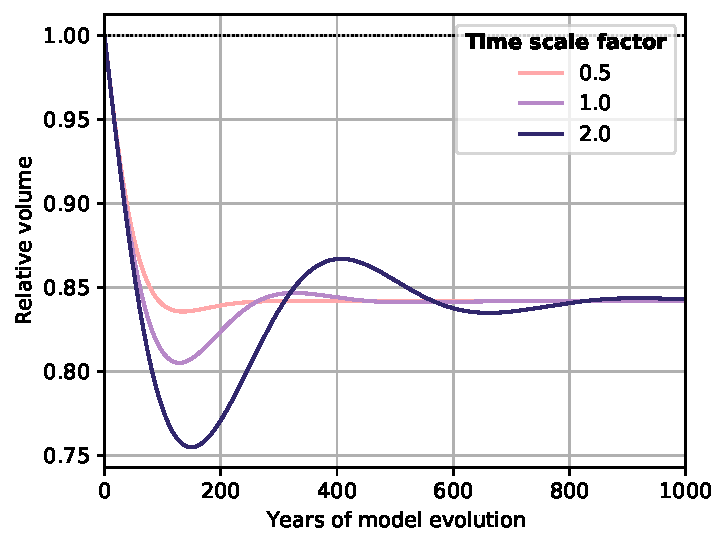
\includegraphics[width=\textwidth]{../plots/final_plots/sensitivity/time_scales_hef.pdf}
      \end{subfigure}
      \hfill
      % HEF scaling params
      \begin{subfigure}[b]{0.476\textwidth}
        \caption{Hintereisferner, different scaling constants}
        \label{fig:sensitivity:scaling_params_hef}
        \centering
        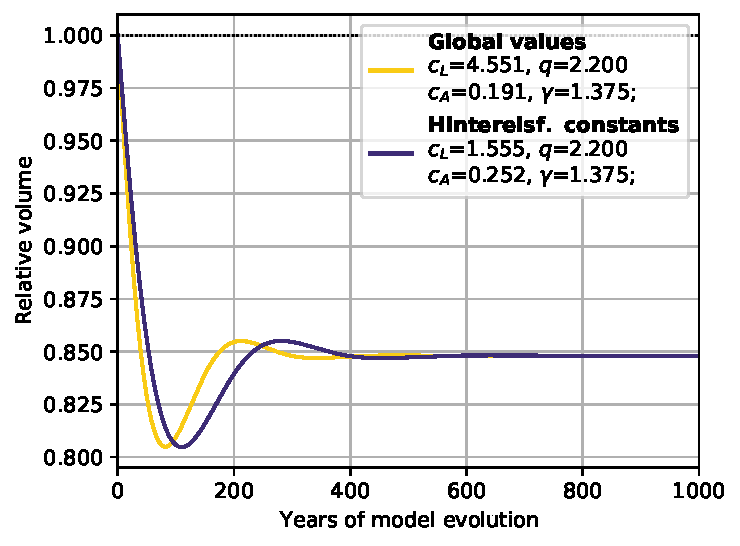
\includegraphics[width=\textwidth]{../plots/final_plots/sensitivity/scaling_params_hef.pdf}
      \end{subfigure}
      
      % HISTALP time scales
      \begin{subfigure}[b]{0.476\textwidth}
        \caption{HISTALP domain, different model-internal time scales}
        \label{fig:sensitivity:time_scales_histalp}
        \centering
        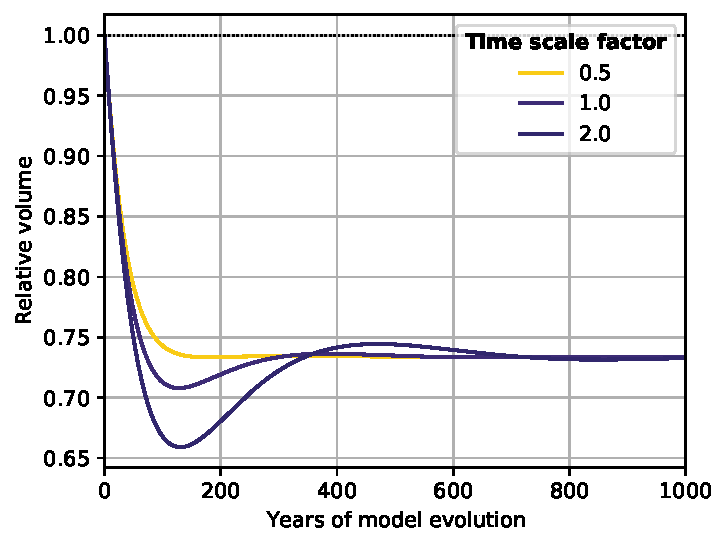
\includegraphics[width=\textwidth]{../plots/final_plots/sensitivity/time_scales_histalp.pdf}
      \end{subfigure}
      \hfill
      % HISTALP scaling params
      \begin{subfigure}[b]{0.476\textwidth}
        \caption{HISTALP domain, different scaling constants and scaling exponents}
        \label{fig:sensitivity:scaling_params_histalp}
        \centering
        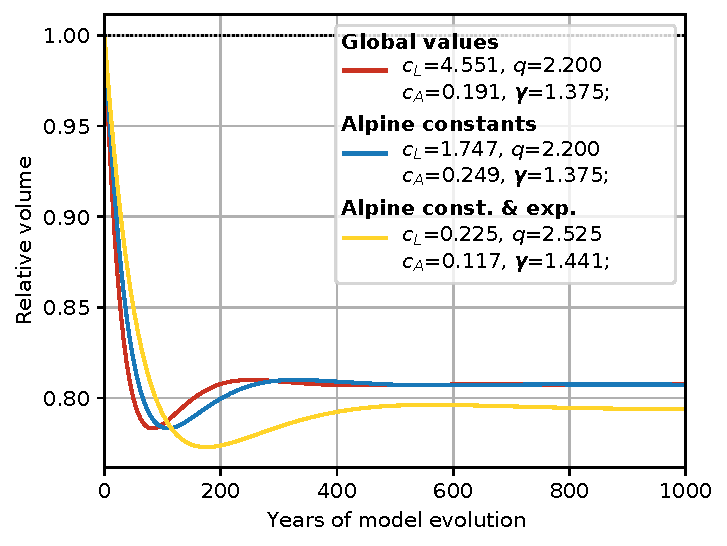
\includegraphics[width=\textwidth]{../plots/final_plots/sensitivity/scaling_params_histalp.pdf}
      \end{subfigure}
      
      \caption{Temporal evolution of glacier ice volume under a positive temperature bias of \SI{+0.5}{\celsius} for the Hintereisferner (RGI60-11.00897) in the two upper panels (\subref{fig:sensitivity:time_scales_hef}) and (\subref{fig:sensitivity:scaling_params_hef}) and for the entire HISTALP domain in the two lower panels (\subref{fig:sensitivity:time_scales_histalp}) and (\subref{fig:sensitivity:scaling_params_histalp}). The right panels show results for different model-internal time scales, scaled by a linear factor (see legend for details). The left panels show results for different scaling constants and scaling exponents (see legend for details). Note the difference in y-axis scales.}
      \label{fig:sensitivity}
    \end{figure}

    \subsection{Sensitivity to scaling parameters} % (fold)
    \label{sec:sensitivity_to_scaling_parameters_results}

      As seen above, the model-internal time scale do not change the absolute values of any geometric glacier property. So what about the scaling parameters? The following paragraph compares the model behavior between the custom Hintereisferner scaling constants and the global scaling constants (Figure\ref{fig:sensitivity:scaling_params_hef}). The scaling exponents are held constant, since it is not possible to compute a linear regression from a single data point. % $c_L = \SI{1.555}{\meter^{3-q}}$ and $c_A = \SI{0.252}{\meter^{3-2\gamma}}$ and the global scaling constants $c_L = \SI{4.551}{\meter^{3-q}}$ and $c_A = \SI{0.191}{\meter^{3-2\gamma}}$.
      Changing the scaling constants leads to different absolute values. As explained in Section~\ref{sub:glacier_evolution_model_implementation}, the \vas{} model starts by computing the initial glacier volume from the surface area via the \vas{} relation. Hence, the initial area stays the same while the initial ice volume increases with the custom scaling constants. The initial volume for the Hintereisferner increases to \SI{0.787}{\cubic\kilo\meter} with custom scaling constants $c_L = \SI{1.555}{\meter^{3-q}}$ and $c_A = \SI{0.252}{\meter^{3-2\gamma}}$, compared to the \SI{0.596}{\cubic\kilo\meter} with the global values. While starting with a larger initial ice volume increases the absolute change in ice volume (\SI{-0.120}{\cubic\kilo\meter} vs. \SI{-0.091}{\cubic\kilo\meter}), it still results in a larger equilibrium ice volume (\SI{0.667}{\cubic\kilo\meter} vs. \SI{0.506}{\cubic\kilo\meter}). However, when normalized with the respective initial ice volumes, the changes in ice volume, the equilibrium values and the overshoots (i.e., minimum values due to the oscillatory behavior) are almost identical (the differences lie far below \SI{0.1}{\percent}). This comes as no surprise, since the scaling constants are canceled out during the normalization process. In fact, when estimating \emph{changes} in regional or global ice volume the scaling constant $c$ can be eliminated altogether \citep[][Section 8.5]{Bahr2015}. While the relative values do not change, the temporal evolution does. As already discussed, the bigger custom scaling constant $c_A$ leads to a bigger initial ice volume. Increasing the glacier's ice volume in turn increases the glacier's response time, since larger glaciers generally react slower to climatic changes. The volume e-folding response time increases to 30 years with the custom scaling constants, compared to 23 years with the global values. The increased response time goes hand in hand with a stronger oscillation. While the amplitude stays the same, the frequency decreases. Hence, the peak of the overshoot shifts by 28 years (to year 100 after the initial climate perturbation) and it takes much longer to reach the new equilibrium state (493 years vs. 371 years).
      While the glacier length reacts analogously to the custom scaling constants, the surface area does not. This was to be expected, since the initial surface area does not depend on the scaling parameters. While the equilibrium value and the e-folding response time are practically not affected, the oscillation amplifies. In addition to the decreased frequency, as for ice volume and glacier length, the surface area overshoots by \SI{15\,761}{\square\meter} more under the custom scaling constants (which corresponds to \SI{\approx0.2}{\percent} of the equilibrium value).
      
      Again, the results of the regional Alpine run (Figure~\ref{fig:sensitivity:scaling_params_histalp}) are analogous to the Hintereisferner test case. While the Hintereisferner test case compares only the global and custom scaling constants, an additional run with custom scaling constants and scaling exponents is investigated. As seen above, changing the scaling constants results in different absolute values (for the initial volume as well as for the final equilibrium volume). However, when normalized with the initial values only the run with custom scaling exponents shows a different (bigger) change in ice volume. The total modeled glacier ice volume shrinks from an initial \SI{229.7}{\cubic\kilo\meter} to a final \SI{182.4}{\cubic\kilo\meter}, subjected to a positive temperature bias of \SI{+0.5}{\celsius}. The change of \SI{-47.3}{\cubic\kilo\meter} corresponds to \SI{-21}{\percent} of the initial value. However, the result does still not compare to the \SI{-47}{\percent} of the flowline model and is not significantly different from the \SI{-19}{\percent} for the other two \vas{} runs.

    % subsection sensitivity_to_scaling_parameters_results (end)

  \section{Projections for the 21st century} % (fold)
  \label{sec:projections_for_the_21st_century}

    This last experiments provides a quantitative estimation of the ice volume change over the 21st century, again comparing the \vas{} model to the flowline model. In addition to the Alps (or much rather the entire RGI region 11, i.e., Central Europe), the experiment runs for all glacier of High Mountain Asia (RGI region 13, 14 and 15, i.e., Central Asia, South Asia West and South Asia East, respectively). The mass balance models are driven by climate data from fifteen different general circulation models\footnote{ BCC-CSM2MR \citep{CMIP6-BCC-CSM2MR}, CAMS-CSM1.0 \citep{CMIP6-CAMS-CSM1.0}, CESM2 \citep{CMIP6-CESM2}, CESM2-WACCM \citep{CMIP6-CESM2-WACCM}, CMCC-CM2-SR5 \citep{CMIP6-CMCC-CM2-SR5}, EC-Earth3 \citep{CMIP6-EC-Earth3}, EC-Earth3-Veg \citep{CMIP6-EC-Earth3-Veg}, FGOALS-f3-L \citep{CMIP6-FGOALS-f3-L}, GFDL-ESM4 \citep{CMIP6-GFDL-ESM4}, INM-CM4-8 \citep{CMIP6-INM-CM4-8}, INM-CM5-0 \citep{CMIP6-INM-CM5-0}, MPI-ESM1.2-HR \citep{CMIP6-MPI-ESM1.2-HR-DKRZ, CMIP6-MPI-ESM1.2-HR-DWD}, MRI-ESM2.0 \citep{CMIP6-MRI-ESM2.0}, NorESM2-MM \citep{CMIP6-NorESM2-MM}, TaiESM1.0 \citep{CMIP6-TaiESM1.0}} (GCMs) from the Coupled Model Intercomparison Project Phase 6 \citep[CMIP6, ][]{Eyring2016_CMIP}, resulting in an ensemble prediction with fifteen members for four different Shared Socioeconomic Pathways (SSP).

    \subsection{Experimental setup} % (fold)
    \label{sub:experimental_setup_projections}

      The inclusion of non Alpine glaciers makes necessitates the use of the global CRU climate dataset. As with the HISTALP dataset before, the \vas{} mass balance model must be calibrated (see Section~\ref{ssub:mb_calib}), which is done using updated global parameters from \citet{Malles2020} ($a = 3, T^\text{melt} = \SI{0}{\celsius}, T^\text{solid precip} = \SI{4}{\celsius}$). The flowline model defaults to the standard OGGM values. To further increase the accuracy of the results, the mass balance residual \bias{} of both models is corrected via the \lstinline`match_regional_geodetic_mb` task, to match the observations presented by \citet{Davaze2020}.

      The 21st century projections are modeled with climate data from fifteen GCMs from CMIP6 for the pathways SSP1-2.6, SSP2-4.5, SSP3-7.0 and SSP5-8.5. The new scenario framework brings together the social development pathways and the Representative Concentration Pathways (RCPS, indicated by the radiative forcing in \si{\watt\per\square\meter} in 2100), or details see \citet{ONeill2016, Riahi2017}.  The GCM data from CMIP6 is prepared using the OGGM task \lstinline`process_cmip_data`, which applies the anomalies to the CRU baseline climate.
      
      The projections start in 2003 (the  observation date of most RGI outlines) and run until 2020 using CRU data, before continuing with the GCM data for the rest of the 21st century. The runs are invoked via the \lstinline`run_from_climate_data`. The presented aggregate ice volumes are normalized with their respective value in 2020 for better comparability.
    
    % subsection experimental_setup (end)

    \subsection{Results} % (fold)
    \label{sub:results_projection}

      % Ich finde die ergebnisse sehr interessant, und sehe ein paar Sachen:
      % - trotz selber Kalibrierung die Ergebisse 2000-2020 tastächlich anders sind
      % - Unterschiede zwischen den Modellen sind schon recht krass, zB in den Alpen

      \begin{figure}[b!]
          \centering
          % VAS Region 11
          \begin{subfigure}[b]{0.476\textwidth}
              \caption{\Vas{} model projection for Central Europe (RGI region 11) }
              \label{fig:cmip:vas_reg_11}
              \centering
              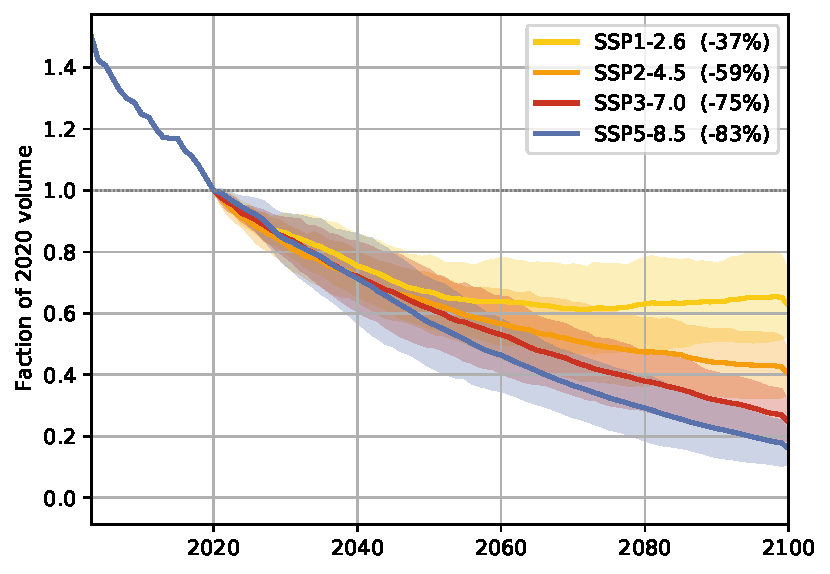
\includegraphics[width=\textwidth]{../plots/final_plots/time_series/cmip/cmip_vas_11.pdf}
          \end{subfigure}
          \hfill
          % Flowline Region 11
          \begin{subfigure}[b]{0.476\textwidth}
              \caption{Flowline model projection for Central Europe (RGI region 11) }
              \label{fig:cmip:fl_reg_11}
              \centering
              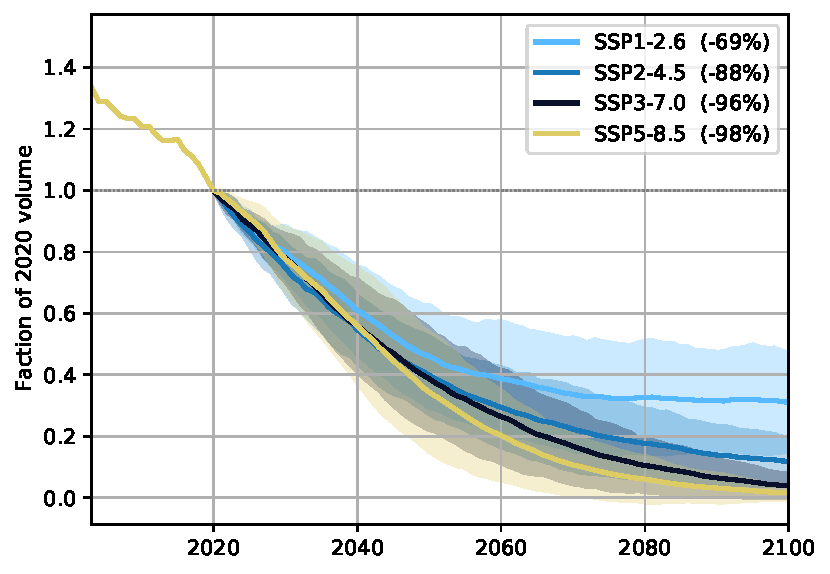
\includegraphics[width=\textwidth]{../plots/final_plots/time_series/cmip/cmip_fl_11.pdf}
          \end{subfigure}

          \caption{Ice volume projection for Central Europe (RGI region 11) using CMIP6 climate data over the 21st century, relative to the year 2020. The left panel shows the result of the volume/area scaling model, the right panel shows the results of the flowline model. Solid lines represent the ensemble average, while the shade represents the $1\sigma$ band. All ensembles have fifteen members. Colors denote different Shared Socioeconomic Pathways, refer to the legend for details. Thereby, the percentage values in parentheses indicate the ice loss relative to 2020.}
          \label{fig:cmip_alps}
      \end{figure}

      Figure~\ref{fig:cmip_alps} shows the ice volume projections for Central Europe (RGI region 11) for the aforementioned SSPs, computed with the \vas{} model in the left panel and the flowline model in the right panel. All percentages are in relation to the 2020 ice volume. Again, both evolution models show qualitatively comparable results, while there are significant quantitative differences.

      The \vas{} model predicts a strong and almost linear decrease in ice volume up to 2020, after which the mass loss attenuates. A new equilibrium is reached only under SSP1-2.6, after an estimated ice loss of $-37\SI{\pm10}{\percent}$. The ensemble average even shows a slight increase over the last 25 years, which most likely stems from the oscillatory behavior of the \vas{} model (cf. Section~\ref{sub:results_test_case} and \ref{sub:results_regional_run}). Under all other SSPs the ice volume is still on a downward trajectory, with an estimated ice loss until 2020 of $-59\SI{\pm6}{\percent}$, $-75\SI{\pm6}{\percent}$, $-83\SI{\pm5}{\percent}$ under SSP2-4.5, SSP3-7.0, SSP5-8.5 respectively. The ice loss predicted by the flowline model ramps up over the initial years, than continues with a rather constant rate before attenuation in the second half of the 21st century and approaching a new equilibrium. The total ice loss amounts to $-68\SI{\pm16}{\percent}$ under SSP1-2.6 and $-88\SI{\pm8}{\percent}$  under SSP2-4.5. For the two SSPs with high forcings the entire glacier ice melts within the margin of error: $-96\SI{\pm4}{\percent}$ under SSP3-7.0 and $-98\SI{\pm2}{\percent}$ under SSP5-8.5.

      Comparing the full simulation period, the \vas{} model generally shows an asymptotic decrease in ice volume while the ice loss predicted by the flowline model follows a sigmoidal shape. Overall, the \vas{} predicts less ice melt than the flowline model, so much so that the final estimates of one model are outside the margin of error of the other. The \vas{} model still shows a downward trajectory for all but the lowest forcing, indicating that \vas{} model reacts slower than the flowline model and may therefore catch up once a new equilibrium is reached. This, however, contradicts all the equilibrium experiments, where the \vas{} model reached its new equilibrium always before the flowline model.

      Focusing on the ``historical'' part from 2003 to 2020, the \vas{} model estimates a total ice volume loss of one third (from \SI{150}{\percent} in 2003 to \SI{100}{\percent} in 2020) while the flowline model estimates a loss of one fourth (from \SI{135}{\percent} in 2003 to \SI{100}{\percent} in 2020).
      The regional average geodetic surface mass balance observations for Central Europe between 2000 and 2020 is \SI{-874}{\milli\metre\waterequivalent\per\year}, while \vas{} model estimates \SI{-1590}{\milli\metre\waterequivalent\per\year} and the flowline model \SI{-1608}{\milli\metre\waterequivalent\per\year}. Those rather large differences show that both models in their respective ``out-of-the-box'' state have difficulties reproducing the mass balance observations for the Alps. Hence, the last calibration step uses \lstinline`match_regional_geodetic_mb` to shift the mass balance residual \bias{} accordingly. This assures that the boundary conditions of both models are as similar as possible and the results as physical as possible. Therefore, the difference between the two models are all the more interesting, showing once more that they do not resolve all the same processes.

      \begin{figure}[htp]

          % VAS Region 13
          \begin{subfigure}[b]{0.476\textwidth}
              \caption{\Vas{} model projection for Central Asia (RGI region 13) }
              \label{fig:cmip:vas_reg_13}
              \centering
              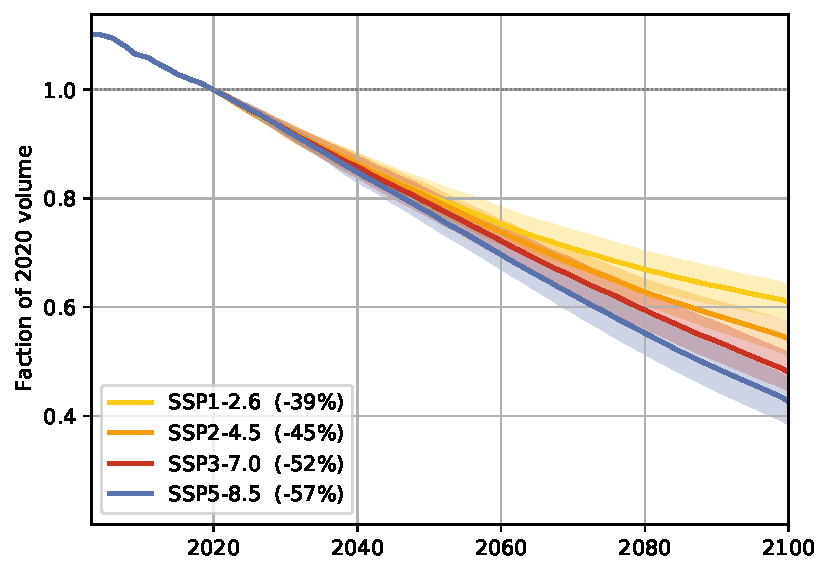
\includegraphics[width=\textwidth]{../plots/final_plots/time_series/cmip/cmip_vas_13.pdf}
          \end{subfigure}
          \hfill
          % Flowline Region 13
          \begin{subfigure}[b]{0.476\textwidth}
              \caption{Flowline model projection for Central Asia (RGI region 13) }
              \label{fig:cmip:fl_reg_13}
              \centering
              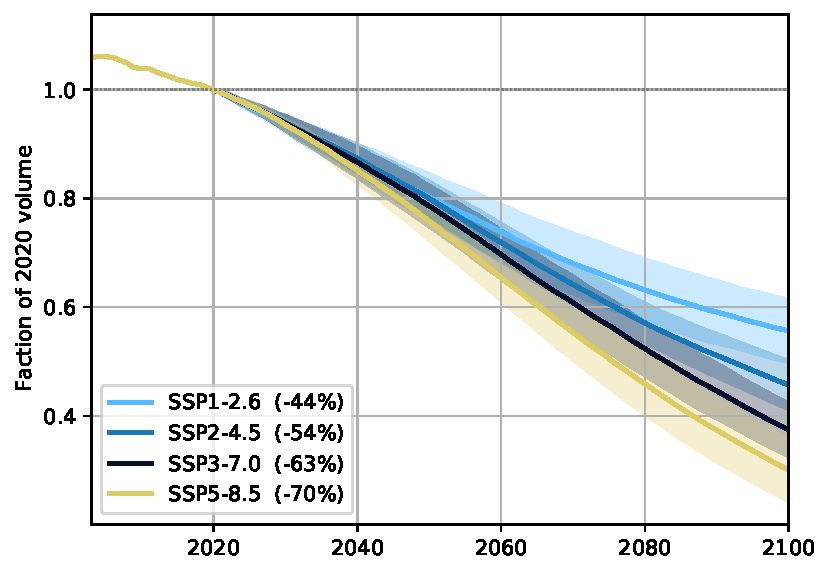
\includegraphics[width=\textwidth]{../plots/final_plots/time_series/cmip/cmip_fl_13.pdf}
          \end{subfigure}

          % VAS Region 14
          \begin{subfigure}[b]{0.476\textwidth}
              \caption{\Vas{} model projection for South Asia West (RGI region 14) }
              \label{fig:cmip:vas_reg_14}
              \centering
              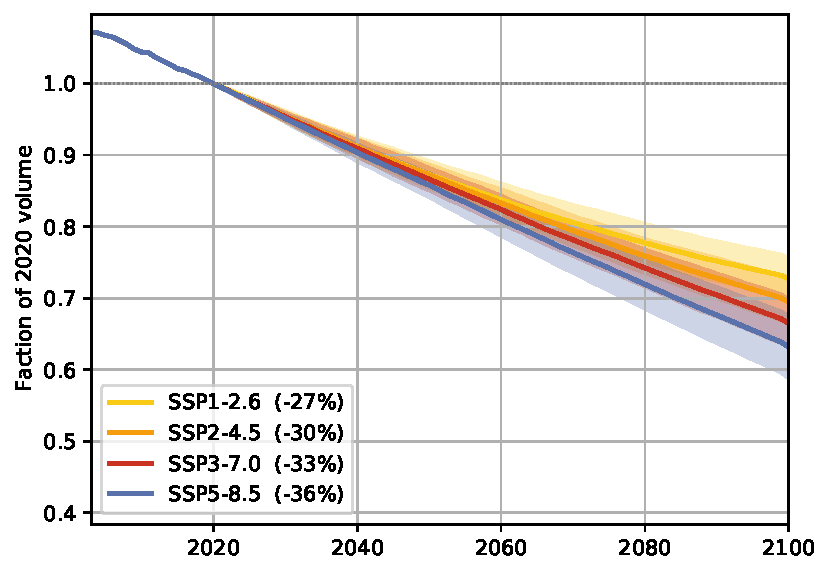
\includegraphics[width=\textwidth]{../plots/final_plots/time_series/cmip/cmip_vas_14.pdf}
          \end{subfigure}
          \hfill
          % Flowline Region 14
          \begin{subfigure}[b]{0.476\textwidth}
              \caption{Flowline model projection for South Asia West (RGI region 14) }
              \label{fig:cmip:fl_reg_14}
              \centering
              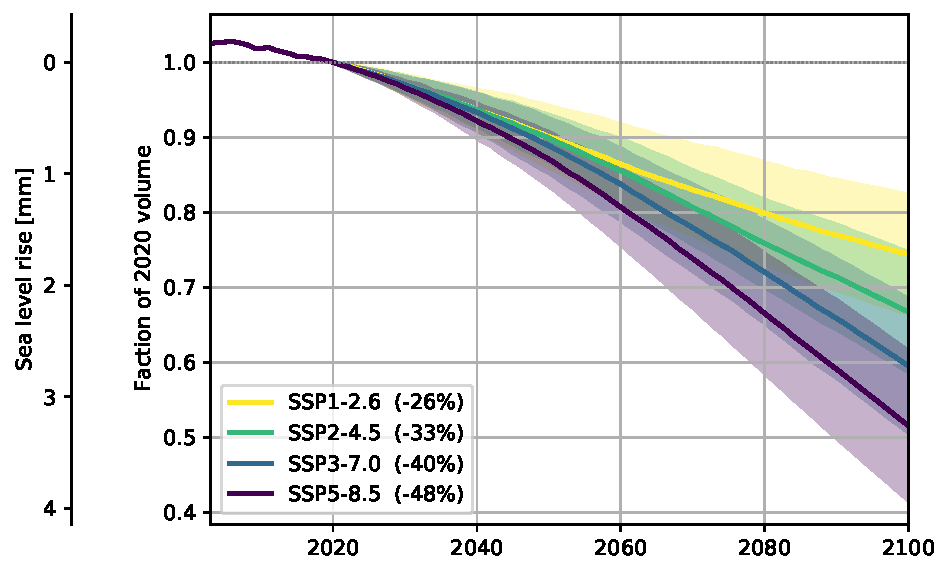
\includegraphics[width=\textwidth]{../plots/final_plots/time_series/cmip/cmip_fl_14.pdf}
          \end{subfigure}

          % VAS Region 15
          \begin{subfigure}[b]{0.476\textwidth}
              \caption{\Vas{} model projection for South Asia East (RGI region 15) }
              \label{fig:cmip:vas_reg_15}
              \centering
              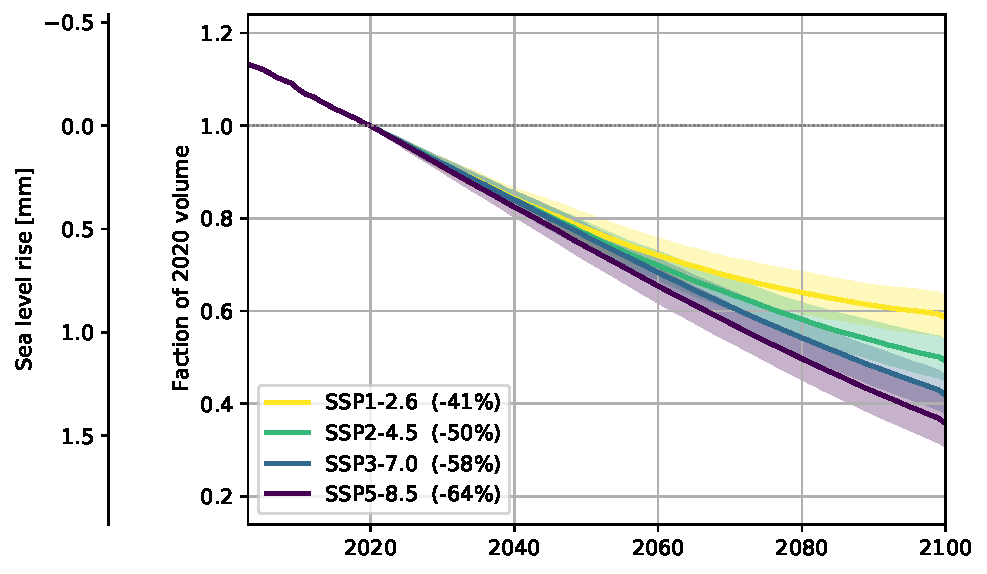
\includegraphics[width=\textwidth]{../plots/final_plots/time_series/cmip/cmip_vas_15.pdf}
          \end{subfigure}
          \hfill
          % Flowline Region 15
          \begin{subfigure}[b]{0.476\textwidth}
              \caption{Flowline model projection for South Asia East (RGI region 15) }
              \label{fig:cmip:fl_reg_15}
              \centering
              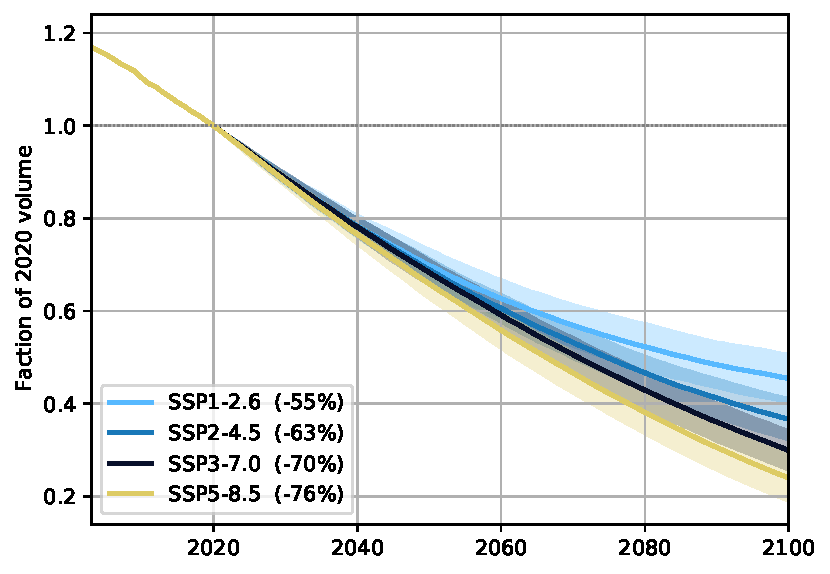
\includegraphics[width=\textwidth]{../plots/final_plots/time_series/cmip/cmip_fl_15.pdf}
          \end{subfigure}

          \caption{As Figure~\ref{fig:cmip_alps}, but for Central Asia (RGI region 13) in the upper panels, South Asia West (RGI region 14) in the middle panels and South Asia East (RGI region 15) in the lower panels.}
          \label{fig:cmip_hma}
      \end{figure}

      \begin{table}[htp]
        \centering
        \small
        \ra{1.3}

        \caption{Ensemble mean and standard deviation of projected ice volume loss in 2100, relative to the ice volume in 2020. \Vas{} model and flowline model are driven by climate data of fifteen GCMs from CMIP6.}
        \label{tab:cmip}
        
        \begin{tabular}{@{}rlrllrl@{}}
          \toprule
          % {} & \phantom{a} & \multicolumn{2}{c}{\textbf{V/A scaling model}} & \phantom{a} & \multicolumn{2}{c}{\textbf{{Flowline model}}} \\
          {} & \phantom{a} & \multicolumn{2}{l}{\textbf{V/A scaling}} & \phantom{a} & \multicolumn{2}{l}{\textbf{Flowline}} \\
          {} & \phantom{a} & \multicolumn{2}{l}{$\overline{\Delta V} \pm \sigma$ [\si{\percent}]} & \phantom{a} & \multicolumn{2}{l}{$\overline{\Delta V} \pm \sigma$ [\si{\percent}]} \\
          \midrule
          \textbf{Central Europe}\\
          SSP1-2.6 & \phantom{a} & -37 & ± 10 & \phantom{a} & -69 & ± 16\\
          SSP2-4.5 & \phantom{a} & -60 & ± 6 & \phantom{a} & -88 & ± 8\\
          SSP3-7.0 & \phantom{a} & -75 & ± 6 & \phantom{a} & -96 & ± 4\\
          SSP5-8.5 & \phantom{a} & -84 & ± 5 & \phantom{a} & -98 & ± 2\\
          \textbf{Central Asia}\\
          SSP1-2.6 & \phantom{a} & -39 & ± 3 & \phantom{a} & -44 & ± 6\\
          SSP2-4.5 & \phantom{a} & -46 & ± 3 & \phantom{a} & -54 & ± 5\\
          SSP3-7.0 & \phantom{a} & -52 & ± 3 & \phantom{a} & -63 & ± 5\\
          SSP5-8.5 & \phantom{a} & -57 & ± 4 & \phantom{a} & -70 & ± 6\\
          \textbf{South Asia East}\\
          SSP1-2.6 & \phantom{a} & -27 & ± 3 & \phantom{a} & -26 & ± 8\\
          SSP2-4.5 & \phantom{a} & -30 & ± 3 & \phantom{a} & -33 & ± 8\\
          SSP3-7.0 & \phantom{a} & -34 & ± 4 & \phantom{a} & -40 & ± 9\\
          SSP5-8.5 & \phantom{a} & -37 & ± 4 & \phantom{a} & -48 & ± 10\\
          \textbf{South Asia West}\\
          SSP1-2.6 & \phantom{a} & -51 & ± 4 & \phantom{a} & -55 & ± 5\\
          SSP2-4.5 & \phantom{a} & -59 & ± 4 & \phantom{a} & -63 & ± 4\\
          SSP3-7.0 & \phantom{a} & -65 & ± 3 & \phantom{a} & -70 & ± 4\\
          SSP5-8.5 & \phantom{a} & -70 & ± 4 & \phantom{a} & -76 & ± 5\\
          \bottomrule
        \end{tabular}
      \end{table}

      Figure~\ref{fig:cmip_hma} shows the 21st century ice volume projections for High Mountain Asia: Central Asia (RGI region 13) in the upper panels, South Asia East (RGI region 14) in the middle panels, South Asia West (RGI region 15) in the lower panels. The overall results are comparable to the simulation for Central Europe. The ensemble averages show an asymptotic or even linear decrease in ice volume for the \vas{} model (with rather narrow uncertainty bands) and a more sigmoidal decrease for the flowline model (with much broader uncertainty bands). The final values of both models are in closer agreement with each other, and are mostly within each others uncertainty bands (see Table~\ref{tab:cmip}). However, the flowline model still predicts more ice loss than the \vas{} model. The differences in estimated ice loss up to 2020 between \vas{} and flowline model are also less pronounced, than for Central Europe. This can possibly be explained by the better agreement between observed and modeled mass balance, the computed differences and following shift of \bias{} range between 177 and \SI{364}{\milli\metre\waterequivalent\per\year}. Furthermore, given the empirical nature of the scaling relations the model performance increases with increasing glacier population size.%\vspace*{1cm}

      % Also wenn ich du wäre würde ich darüber noch diskutieren.
      % Und ich wurde vielleicht noch regional ein bisschen unterscheiden zwischen Gletschern des oberer und unteren Quartils (bezogen auf Fläche), um zu sehen ob die ‘model response’ anders ist

      Finally, the model response is investigated as a function of initial glacier surface area. The glaciers of each region are divided in two size classes, above and below the 95th percentiles in RGI area (see Table~\ref{tab:area_percentile} for details). While the regions have different distributions of glacier sizes, the area thresholds for all regions are in the same order of magnitude (\SI{\approx 3}{\square\kilo\meter}) and the aggregate area of the upper \SI{5}{\percent} of glaciers amounts to more than half of the total area (between \SI{52}{\percent} and \SI{66}{\percent}).

      \begin{figure}[htp]

          % VAS Region 11
          \begin{subfigure}[b]{0.476\textwidth}
              \caption{\Vas{} model projection for Central Europe (RGI region 11) }
              \label{fig:cmip:area_classes_reg_11}
              \centering
              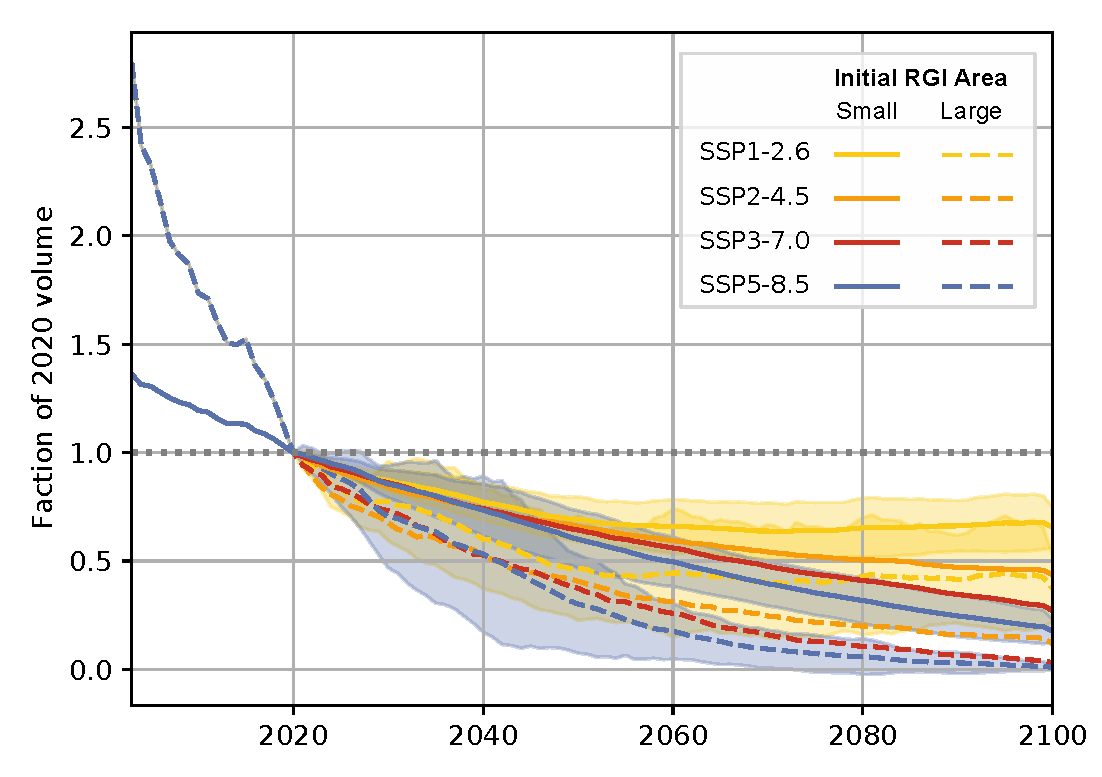
\includegraphics[width=\textwidth]{../plots/final_plots/time_series/cmip/area_classes_vas_11.pdf}
          \end{subfigure}
          \hfill
          % Flowline Region 11
          \begin{subfigure}[b]{0.476\textwidth}
              \caption{Flowline model projection for Central Europe (RGI region 11) }
              \label{fig:cmip:area_classes_11}
              \centering
              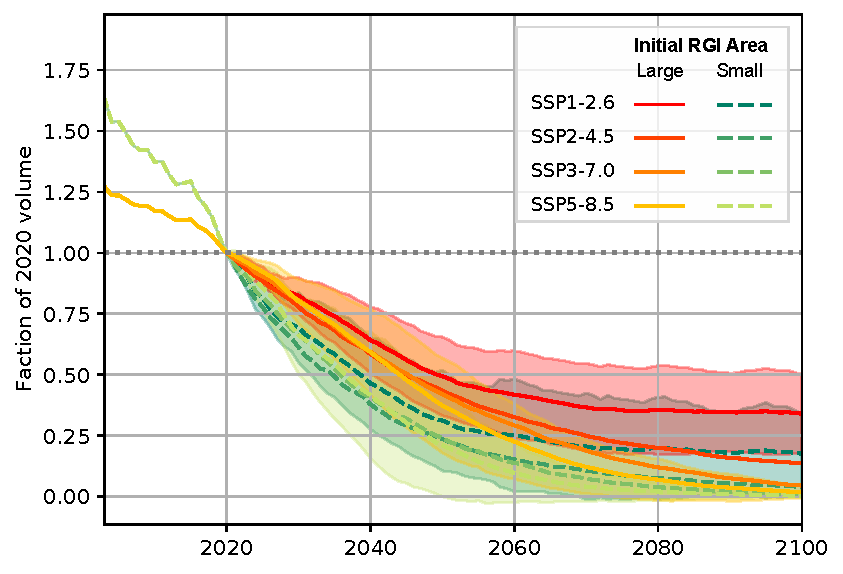
\includegraphics[width=\textwidth]{../plots/final_plots/time_series/cmip/area_classes_fl_11.pdf}
          \end{subfigure}

          \vspace*{0.5cm}

          % VAS Region 14
          \begin{subfigure}[b]{0.476\textwidth}
              \caption{\Vas{} model projection for South Asia West (RGI region 14) }
              \label{fig:cmip:area_classes_reg_14}
              \centering
              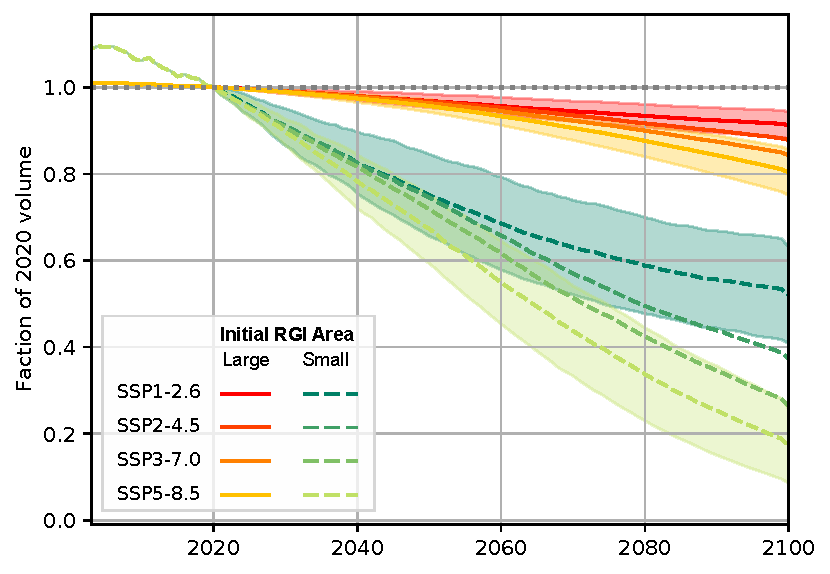
\includegraphics[width=\textwidth]{../plots/final_plots/time_series/cmip/area_classes_vas_14.pdf}
          \end{subfigure}
          \hfill
          % Flowline Region 14
          \begin{subfigure}[b]{0.476\textwidth}
              \caption{Flowline model projection for South Asia West (RGI region 14) }
              \label{fig:cmip:area_classes_14}
              \centering
              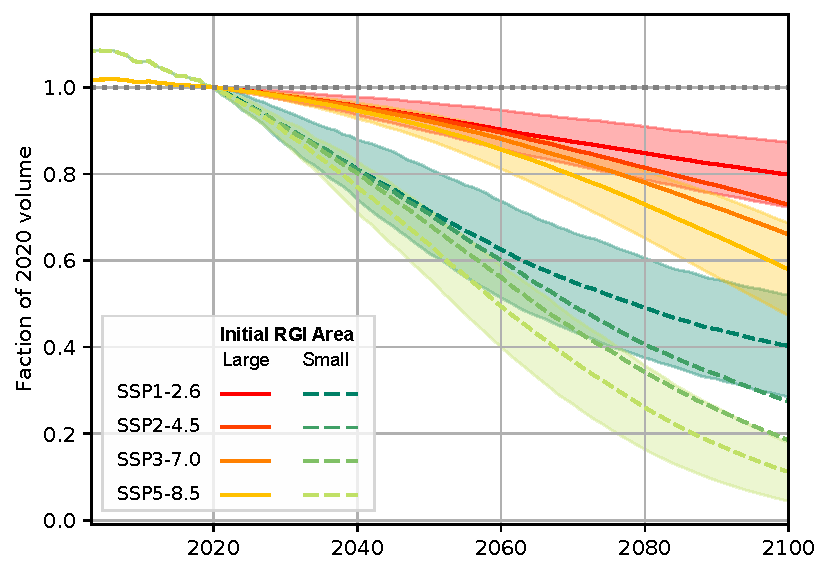
\includegraphics[width=\textwidth]{../plots/final_plots/time_series/cmip/area_classes_fl_14.pdf}
          \end{subfigure}

          \vspace*{0.5cm}

          \caption{As Figure~\ref{tab:cmip} for Central Europe (upper panels) and South Asia West (lower panels), but distinguishing between small glaciers (dashed lines) and large glaciers (solid lines). Small glaciers are all glaciers below the 95th percentile in RGI start area, large glacier all glaciers above. Uncertainty bands are only shown for SSP1 and SSP5.}
          \label{fig:cmip_area_classes}
      \end{figure}

      Figure~\ref{fig:cmip_area_classes} shows the 21st century volume projections distinguishing between small and large glaciers for Central Europe and South Asia West. There are no unexpected results: the smaller glacier loose more ice volume relative to 2020 in less time; the flowline model shows less differences in ice loss between the two size classes than the \vas{} model. The same holds true for Central Asia and South Asia East (not shown). The differences in ice volume evolution between the two size classes are much larger for High Mountain Asia than for Central Europe. This indicates that glacier size does matter, however mostly for very large glaciers. South Asia West has about seven times more glaciers than Central Europe, but almost eighteen times the surface area in the larger size class (in addition to an already higher 95th percentile, see Table~\ref{tab:area_percentile}).

      The small glaciers modeled by the \vas{} model loose considerably more ice volume before 2020, than the large ones. For example, the estimated ice loss for Central Europe between 2003 and 2020 amounts to \SI{64}{\percent} (i.e., from \SI{280}{\percent} to \SI{100}{\percent}) for the small glaciers, while under SSP1-2.6 and SSP2-4.5 some ice persists throughout the rest of the 21st century. However, since the glaciers in Central Europe are overall smaller, there is generally less difference in projected ice volume between the two size classes compared to High Mountain Asia (true for the \vas{} model and flowline model.)

      \vspace*{1cm}

      \begin{table}[htp]
        \centering
        \small
        \ra{1.4}

        \caption{Number of glaciers and total surface area of the lower \SI{95}{\percent} and upper \SI{95}{\percent}  of RGI area, additional the threshold area, i.e. the 95th percentile, is given.}
        \label{tab:area_percentile}
          
        \begin{tabular}{@{}rlrrlclrr@{}}
          \toprule
          {} & \phantom{a} & \multicolumn{2}{c}{\textbf{Lower \SI{95}{\percent}}} & \phantom{a} & \textbf{Threshold} & \phantom{a} & \multicolumn{2}{c}{\textbf{Upper \SI{5}{\percent}}} \\
          {} & {} & $n_\text{Glaciers}$ & $\sum A$ [\si{\square\kilo\meter}] & {} & $A$ [\si{\square\kilo\meter}] & {} & $n_\text{Glaciers}$ & $\sum A$ [\si{\square\kilo\meter}] \\
          \midrule
          \textbf{Central Europe} & & 3730 & 831 & & 2.15 & & 197 & 1261 \\
          \textbf{Central Asia} & & 51707 & 21460 & & 2.96 & & 2722 & 27844 \\
          \textbf{South Asia West} & & 26588 & 11490 & & 3.46 & & 1400 & 22079 \\
          \textbf{South Asia East} & & 12463 & 7066 & & 4.10 & & 656 & 7668 \\

          \bottomrule
        \end{tabular}
      \end{table}

    
    % subsection results (end)
  
  % section projections_for_the_21st_century (end)